\section{Veränderungen}
\subsection{Klassendiagramm}
Im Folgenden wird anhand des aktualisierten Klassendiagramms gezeigt, was sich zum Entwurf verändert hat.

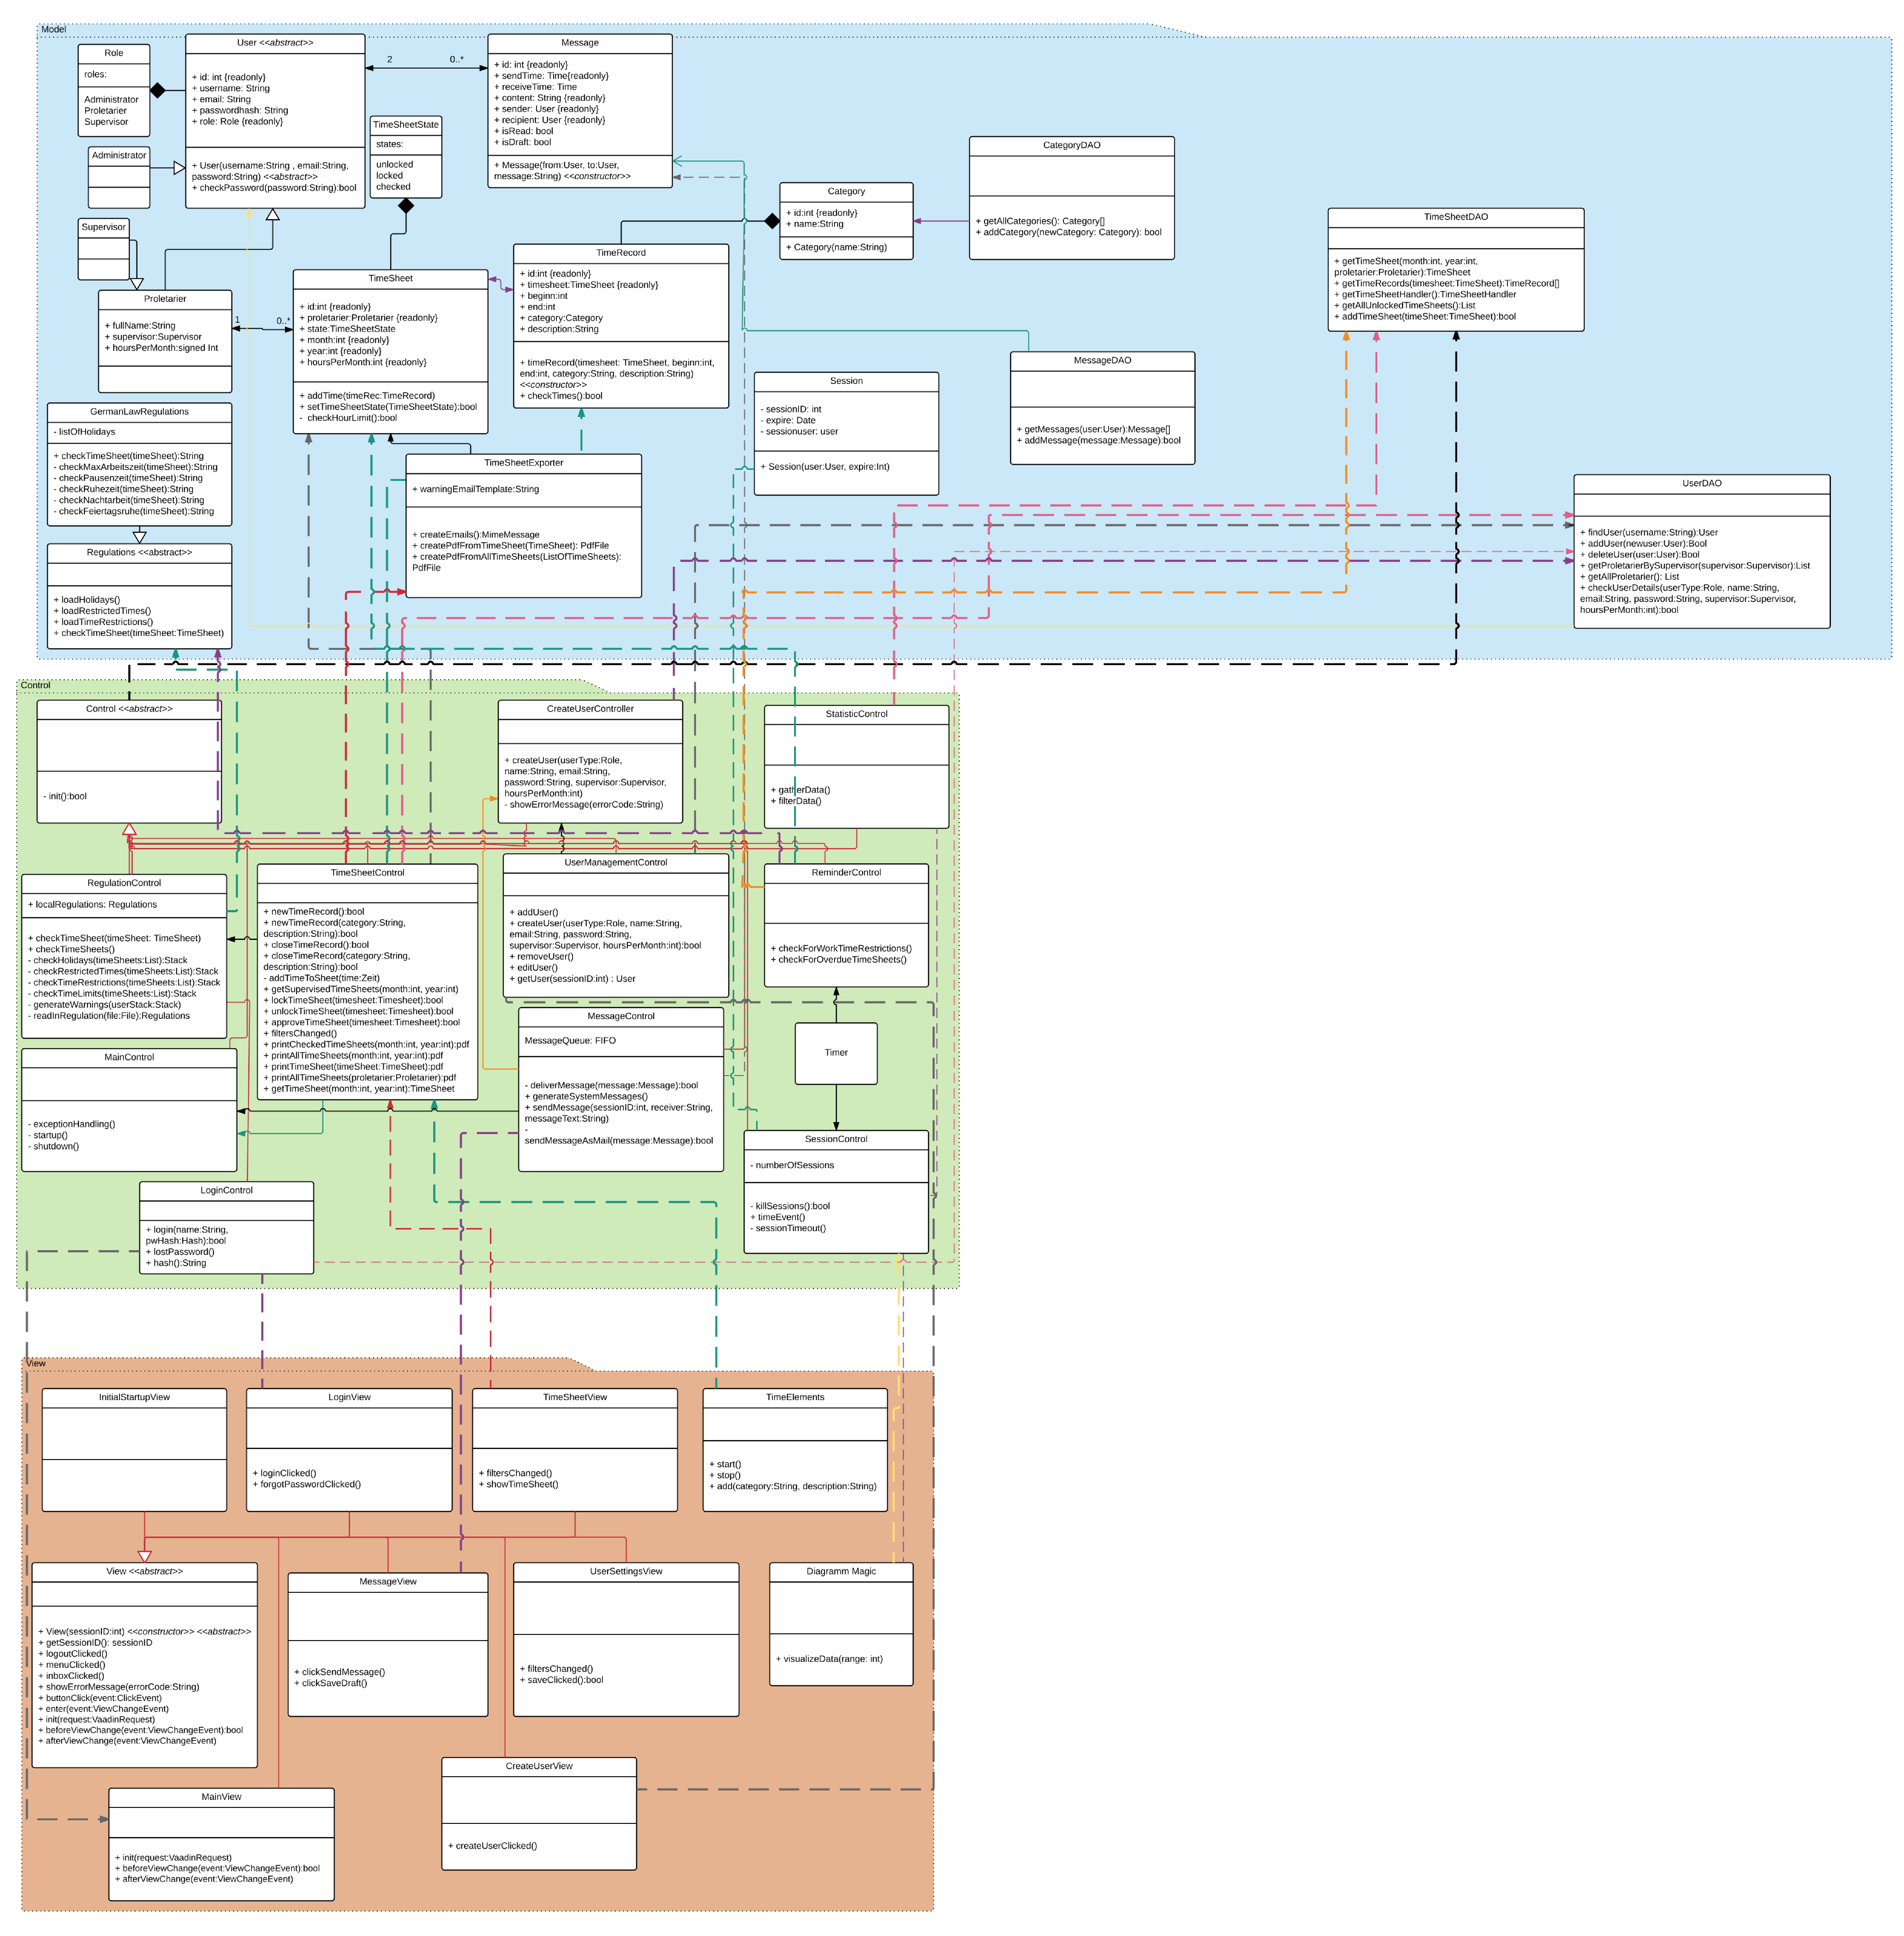
\includegraphics{Class-Diagramm_alt.pdf}
In der view haben sich folgenden Änderungen ergeben:
\VerbatimInput{view-diff}

In der conrtol haben sich folgende Änderungen ergeben:
\VerbatimInput{control-diff}
Im model haben sich folgende Änderungen ergeben: %TODO tex syntax
\VerbatimInput{model-diff}
Daraus ergibt sich das aktualisierte Klassendiagramm:

%neues Klassendiagramm

\subsection{Sequenzen}
Die Sequenzdiagramme aus dem Entwurfen haben sich wie folgt verändert:
\subsubsection{Login Sequenz}

    \begin{figure}
      \centering
        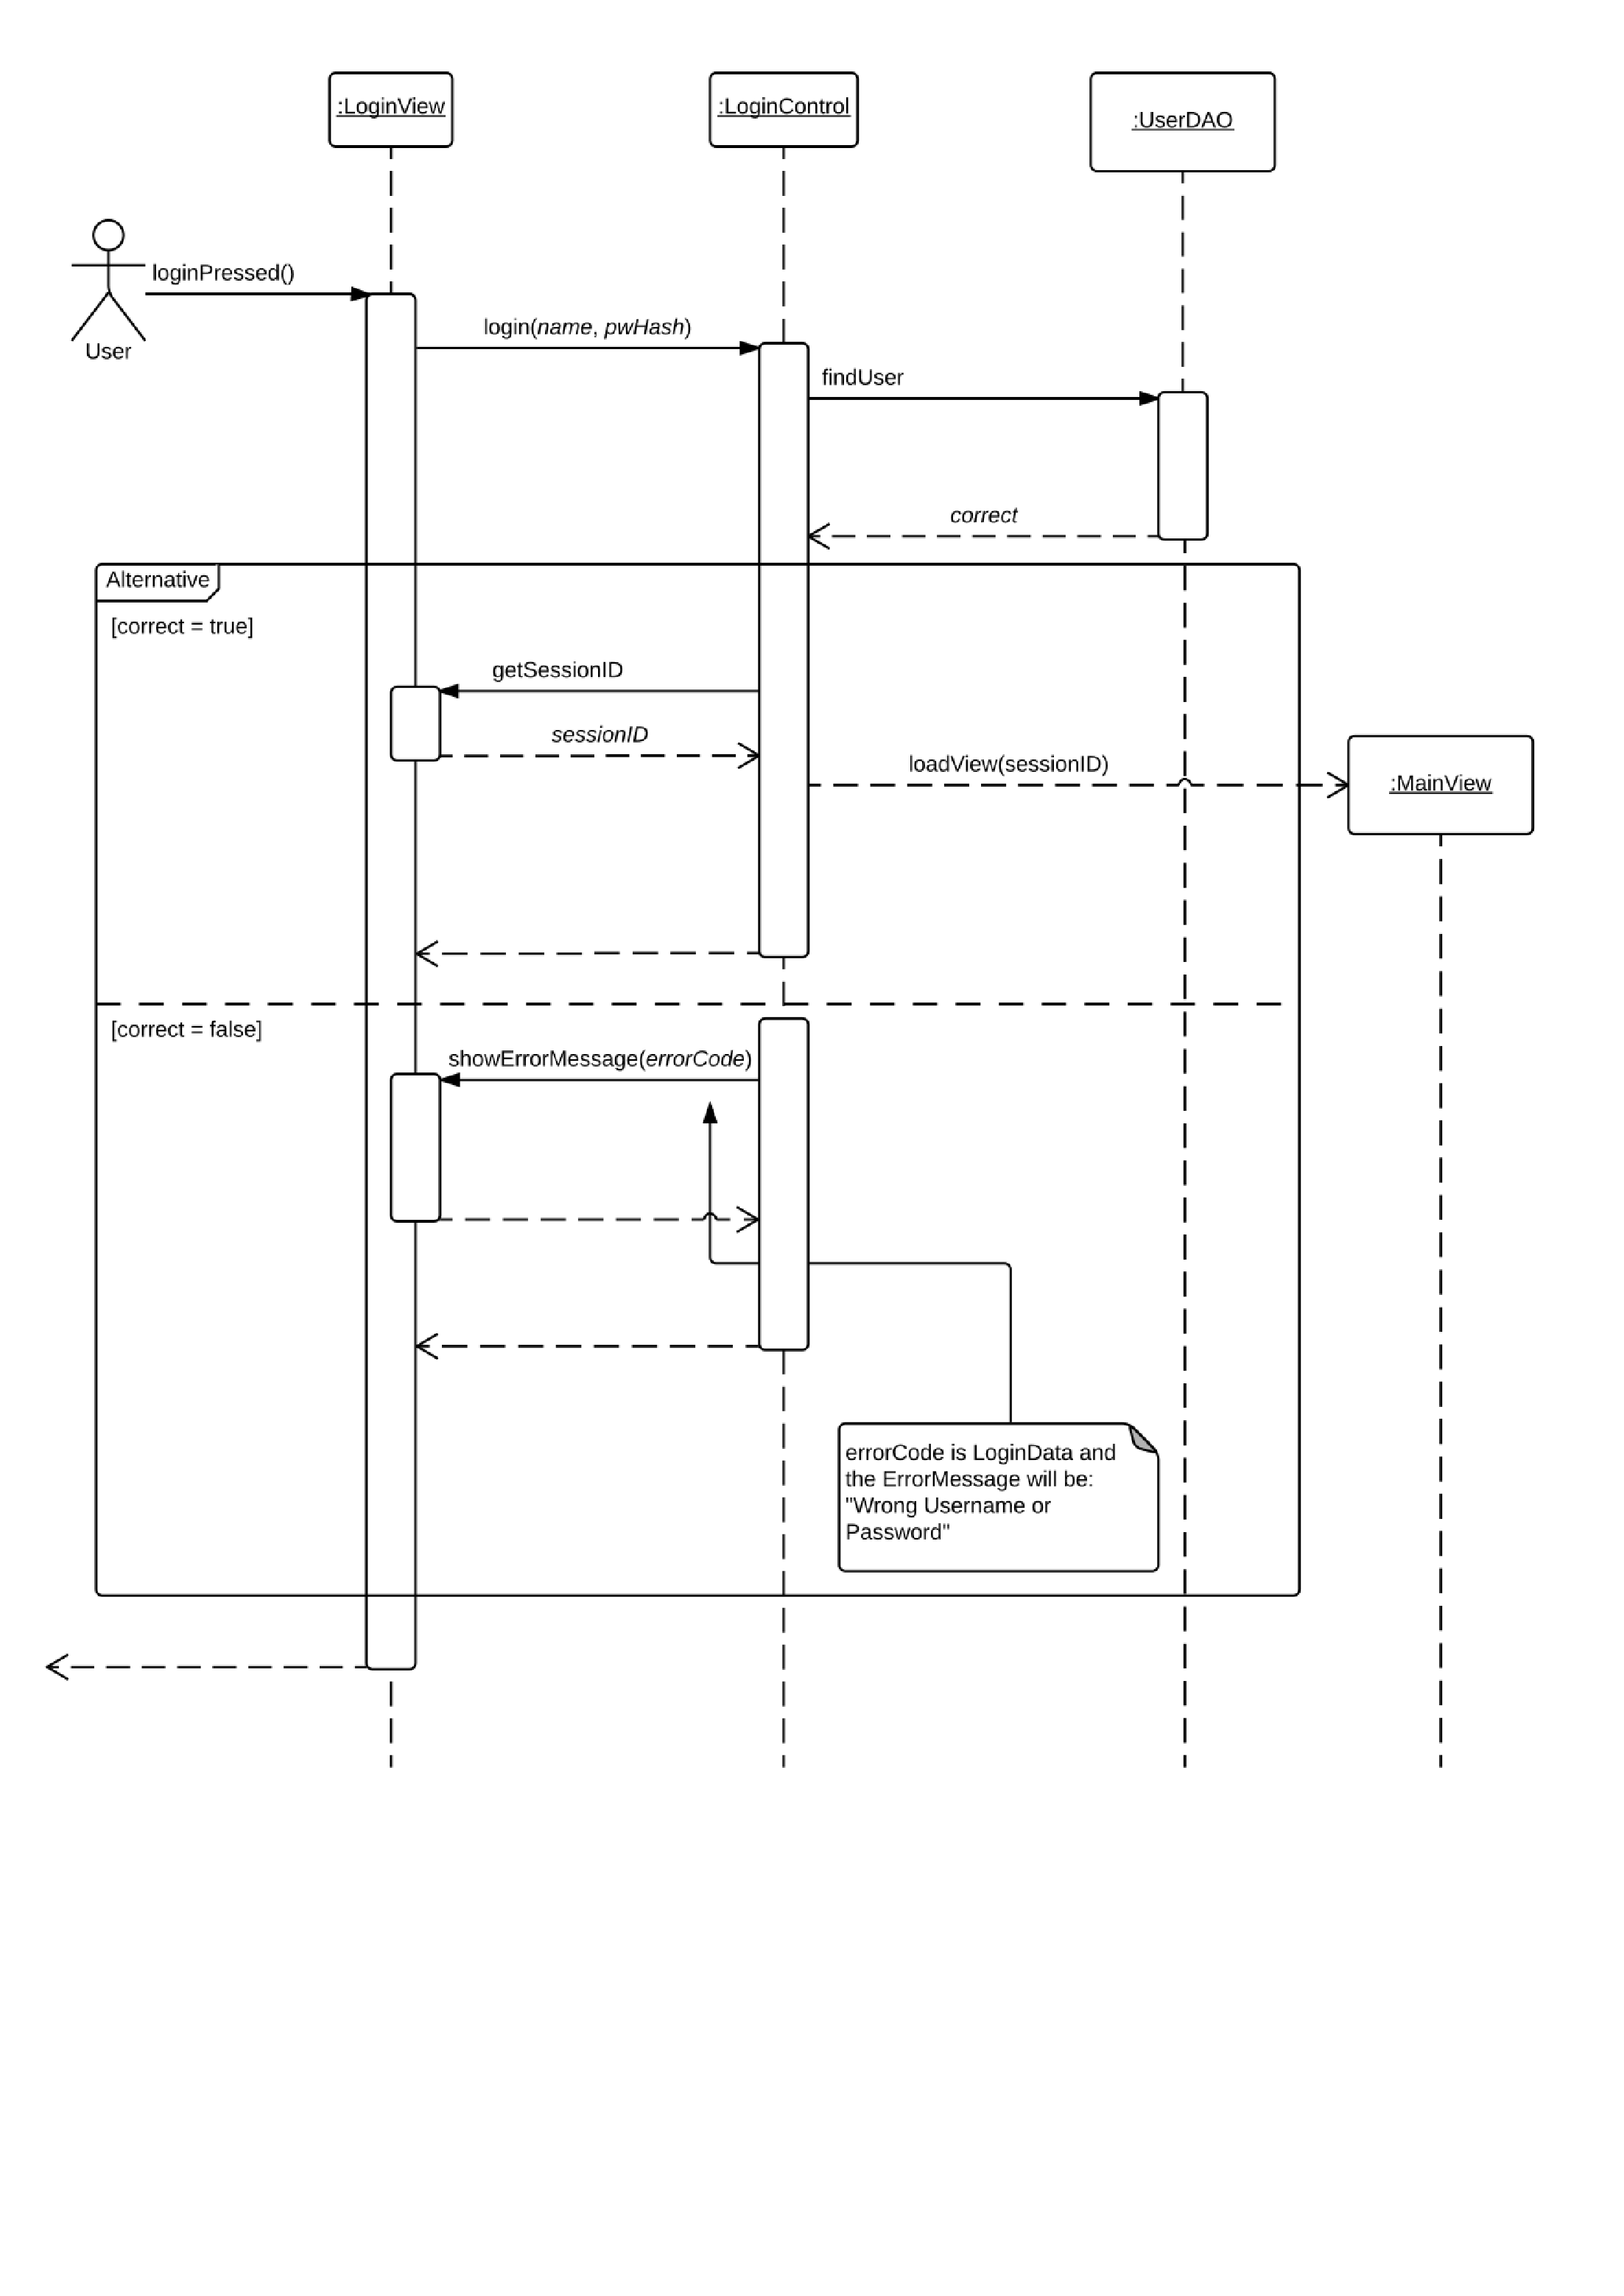
\includegraphics[width=\linewidth]{Login-Sequenz.pdf}
       \caption{Alte Login Sequenz}
    \end{figure}

    \paragraph{Veränderungen}
        \begin{itemize}
            \item Login wurde um die Funktion \emph{remember me} erweitert.
            \item Die Authentifizierung wurde in einklang mit dem Shiro Framework gestaltet:
            \begin{itemize}
                \item Zum Login wird ein token aus Passwort und Username genutzt.
                \item Durch das Token wird der Nutzer ermittelt und dessen Authentifizierungsdaten\(Password, ...\) geholt.
                \item Diese werden mittels einen speziellen Hash vergleicher mit dem angegebenen Token verglichen.
            \end{itemize}
            \item Laden der View wurde durch Vaadins \emph{navigateTo} ersetzt.
        \end{itemize}

    \begin{figure}
      \centering
        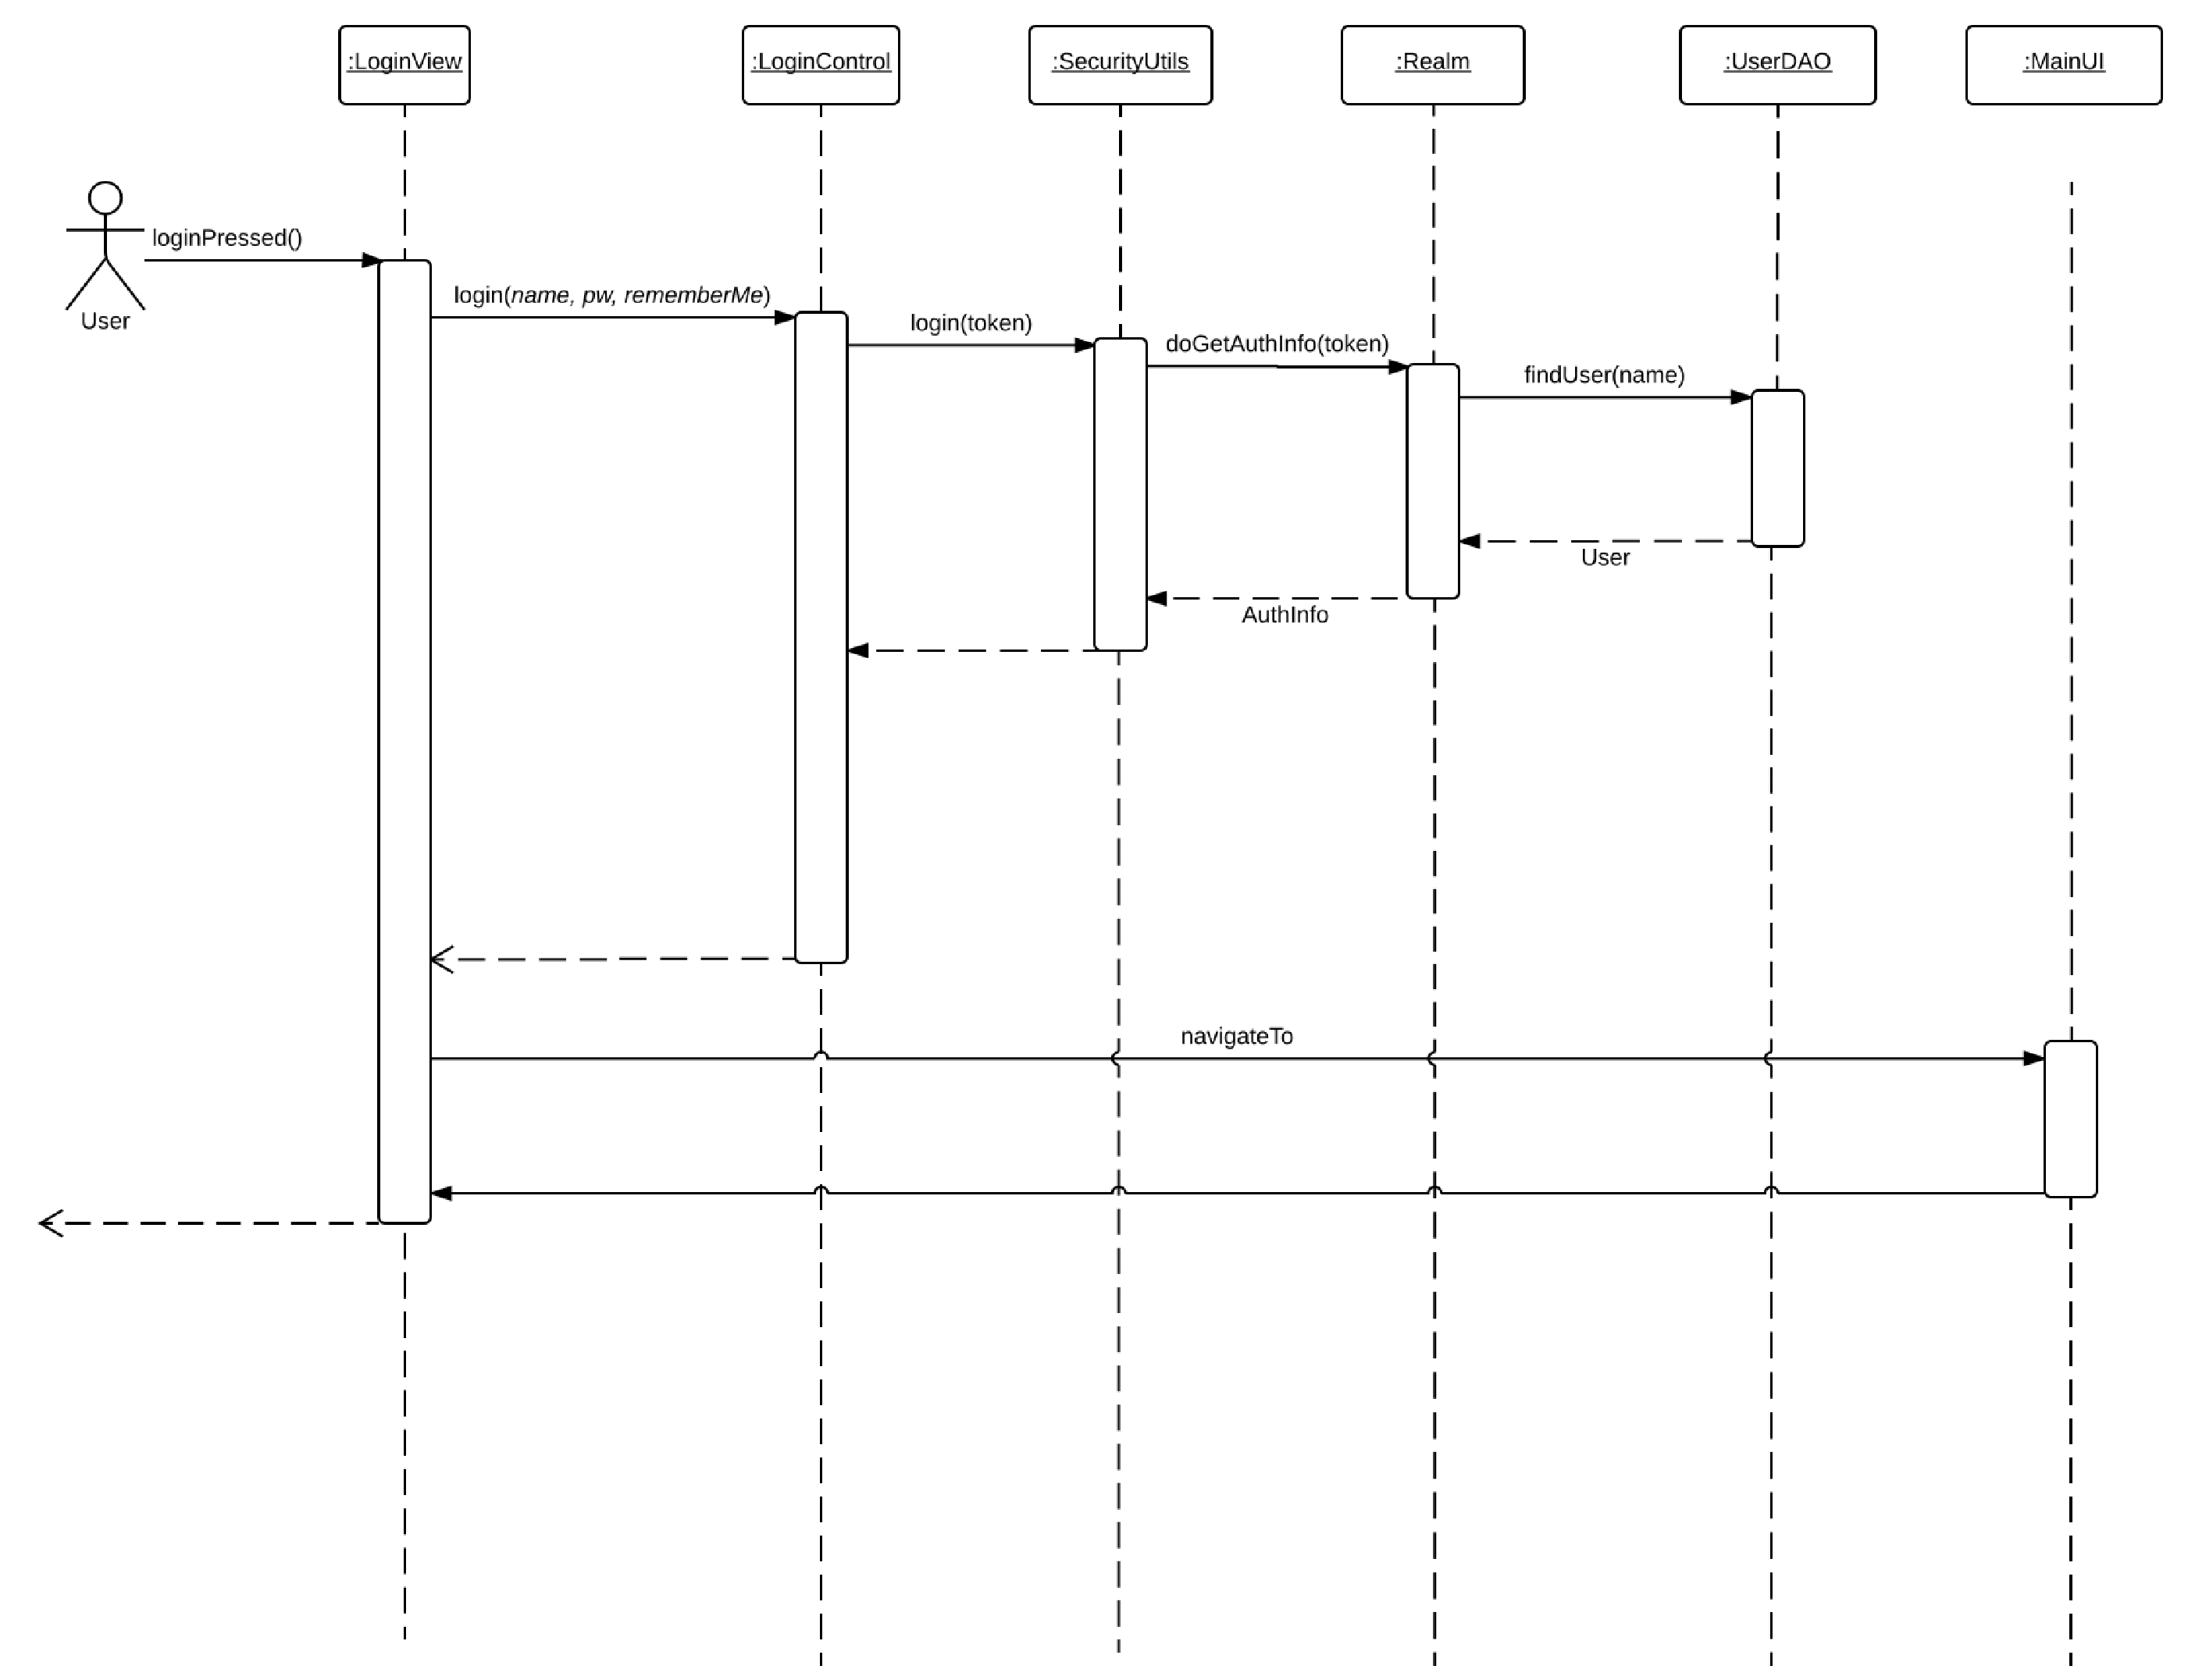
\includegraphics[width=\linewidth]{Login-Sequenz-new.pdf}
       \caption{Neue Login Sequenz}
    \end{figure}

    \subsection{Account erstellungs Sequenz}

    \begin{figure}
      \centering
        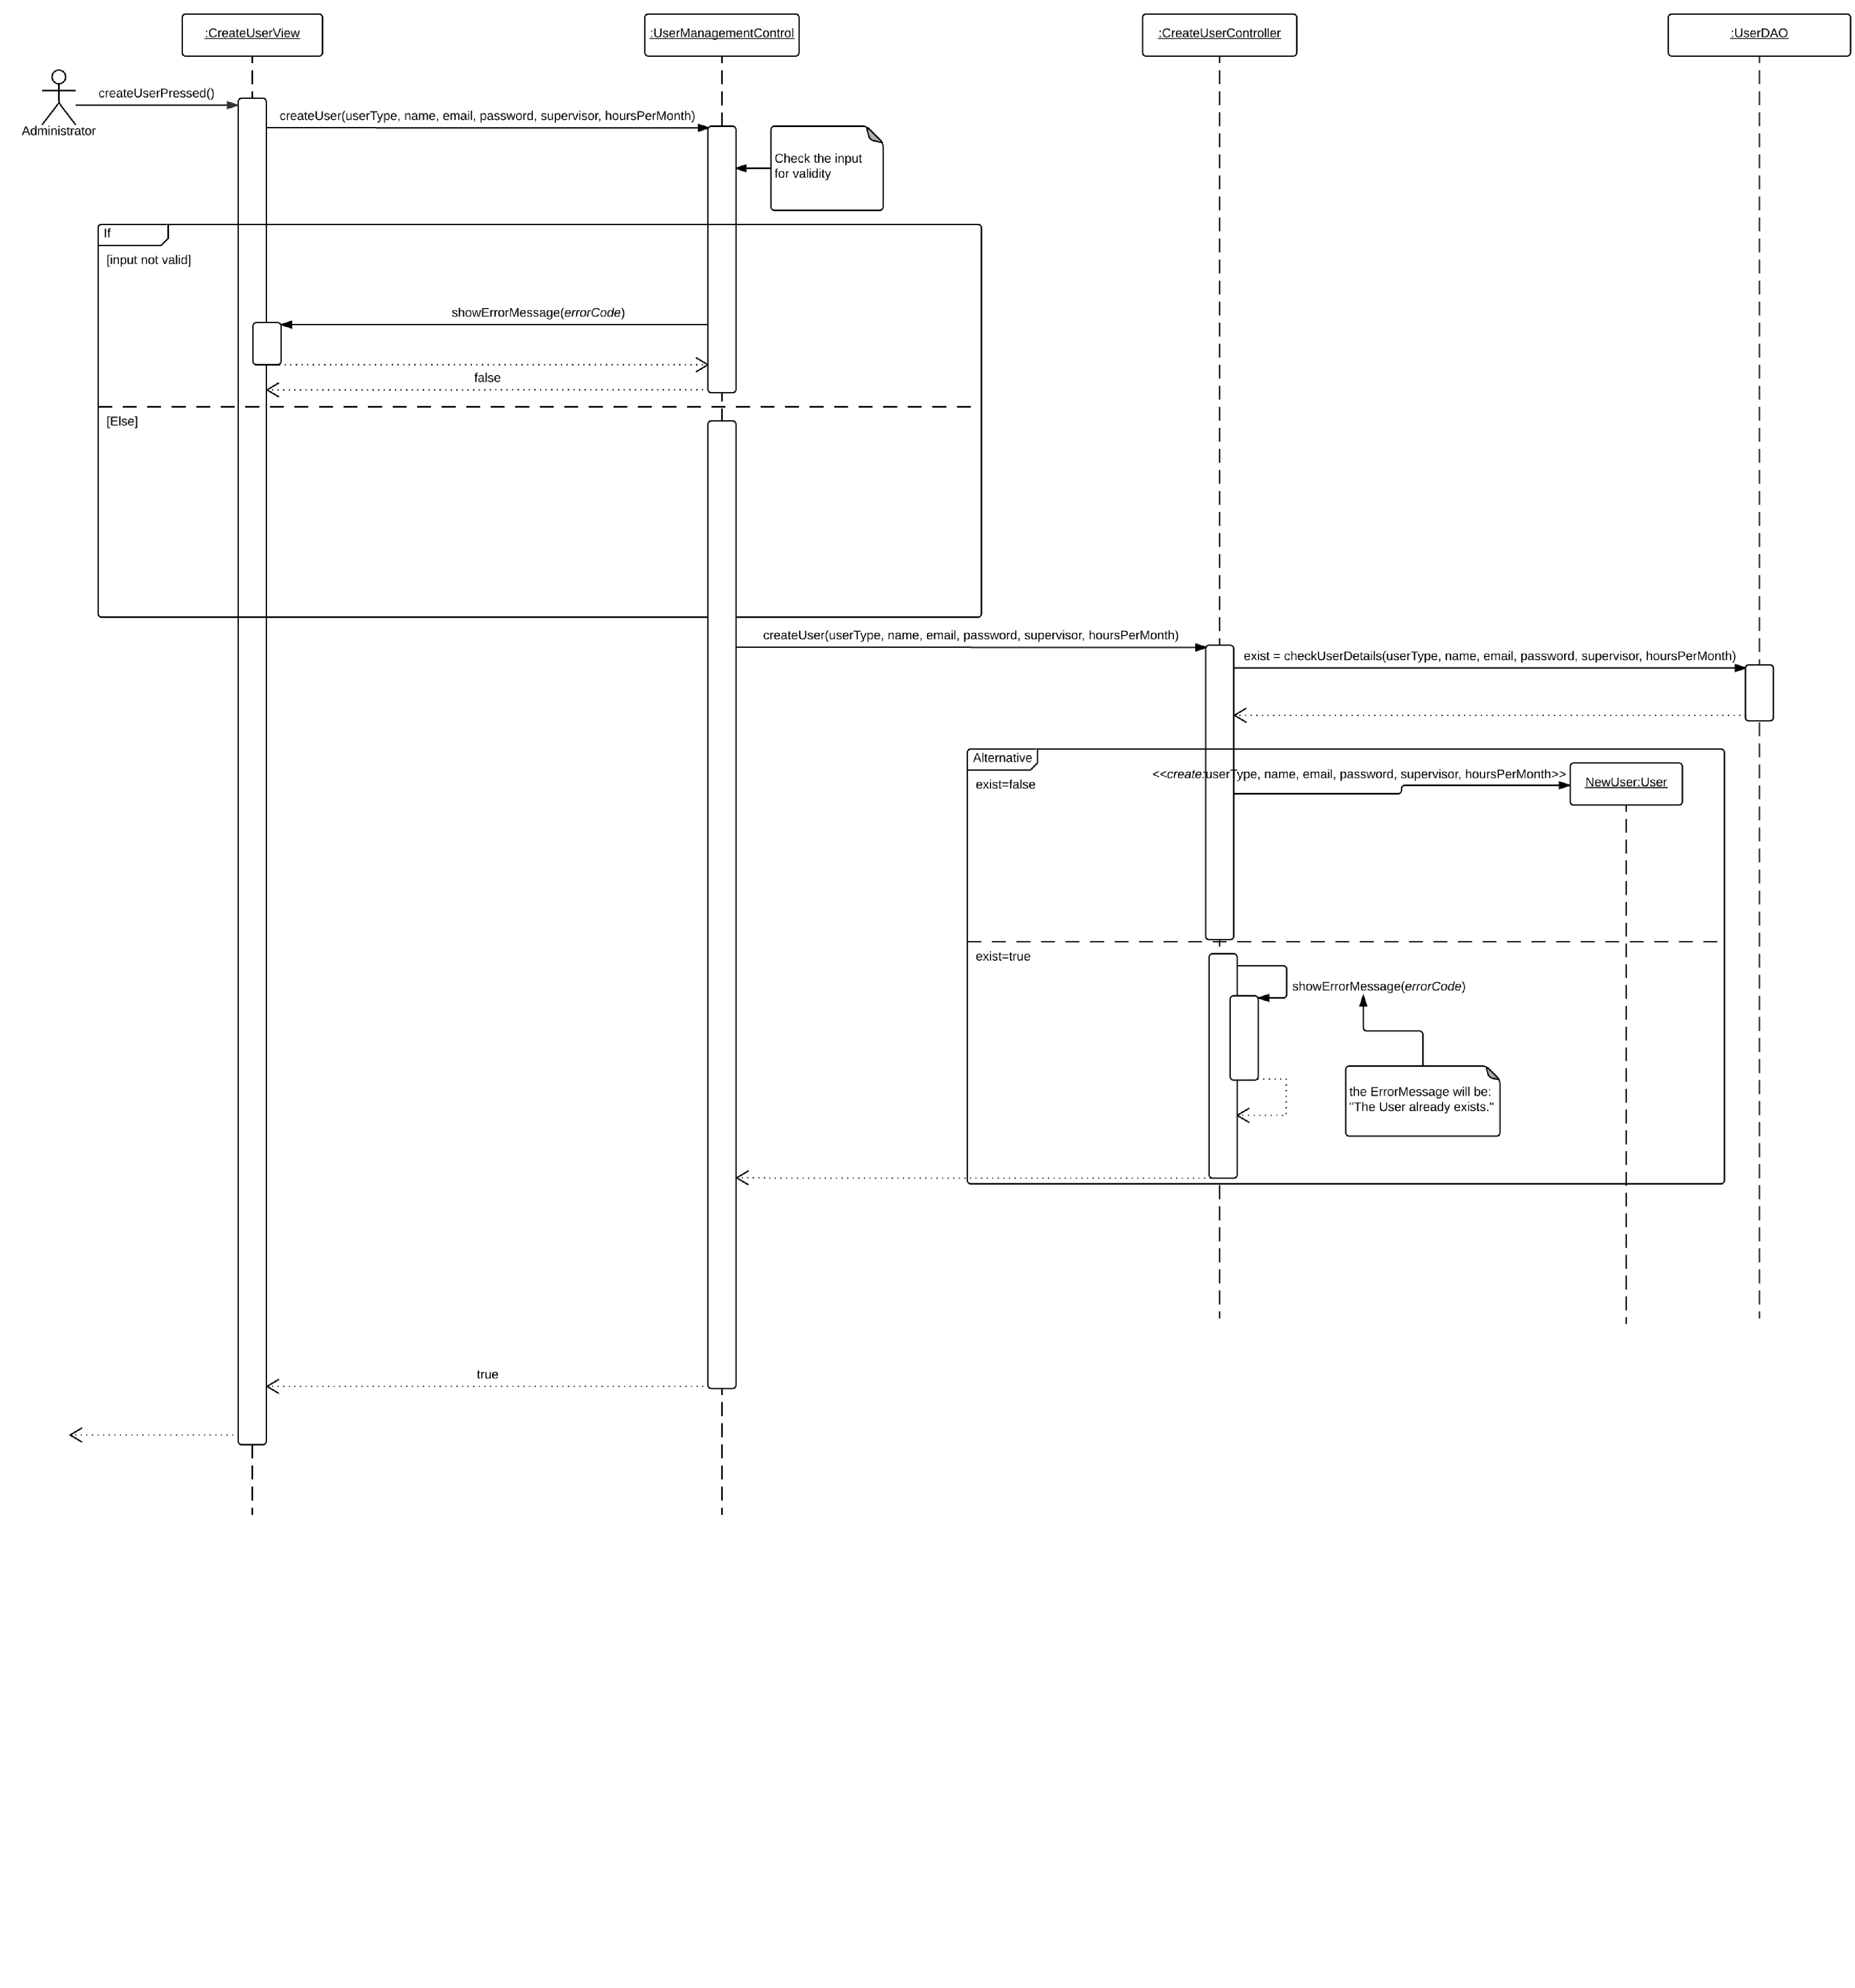
\includegraphics[width=\linewidth]{Create-user-account.pdf}
       \caption{alte Benutzererstellungssequenz}
    \end{figure}

    \paragraph{Veränderungen}
        \begin{itemize}
            \item Der Ablauf wurde vereinfacht. Es wird nurnoch die CreateUserControl Klasse angespochen.
            \item Überprüfungen wurden durch eine verbesserte klarere interne Exception Struktur vereinfacht.
        \end{itemize}

    \begin{figure}
      \centering
        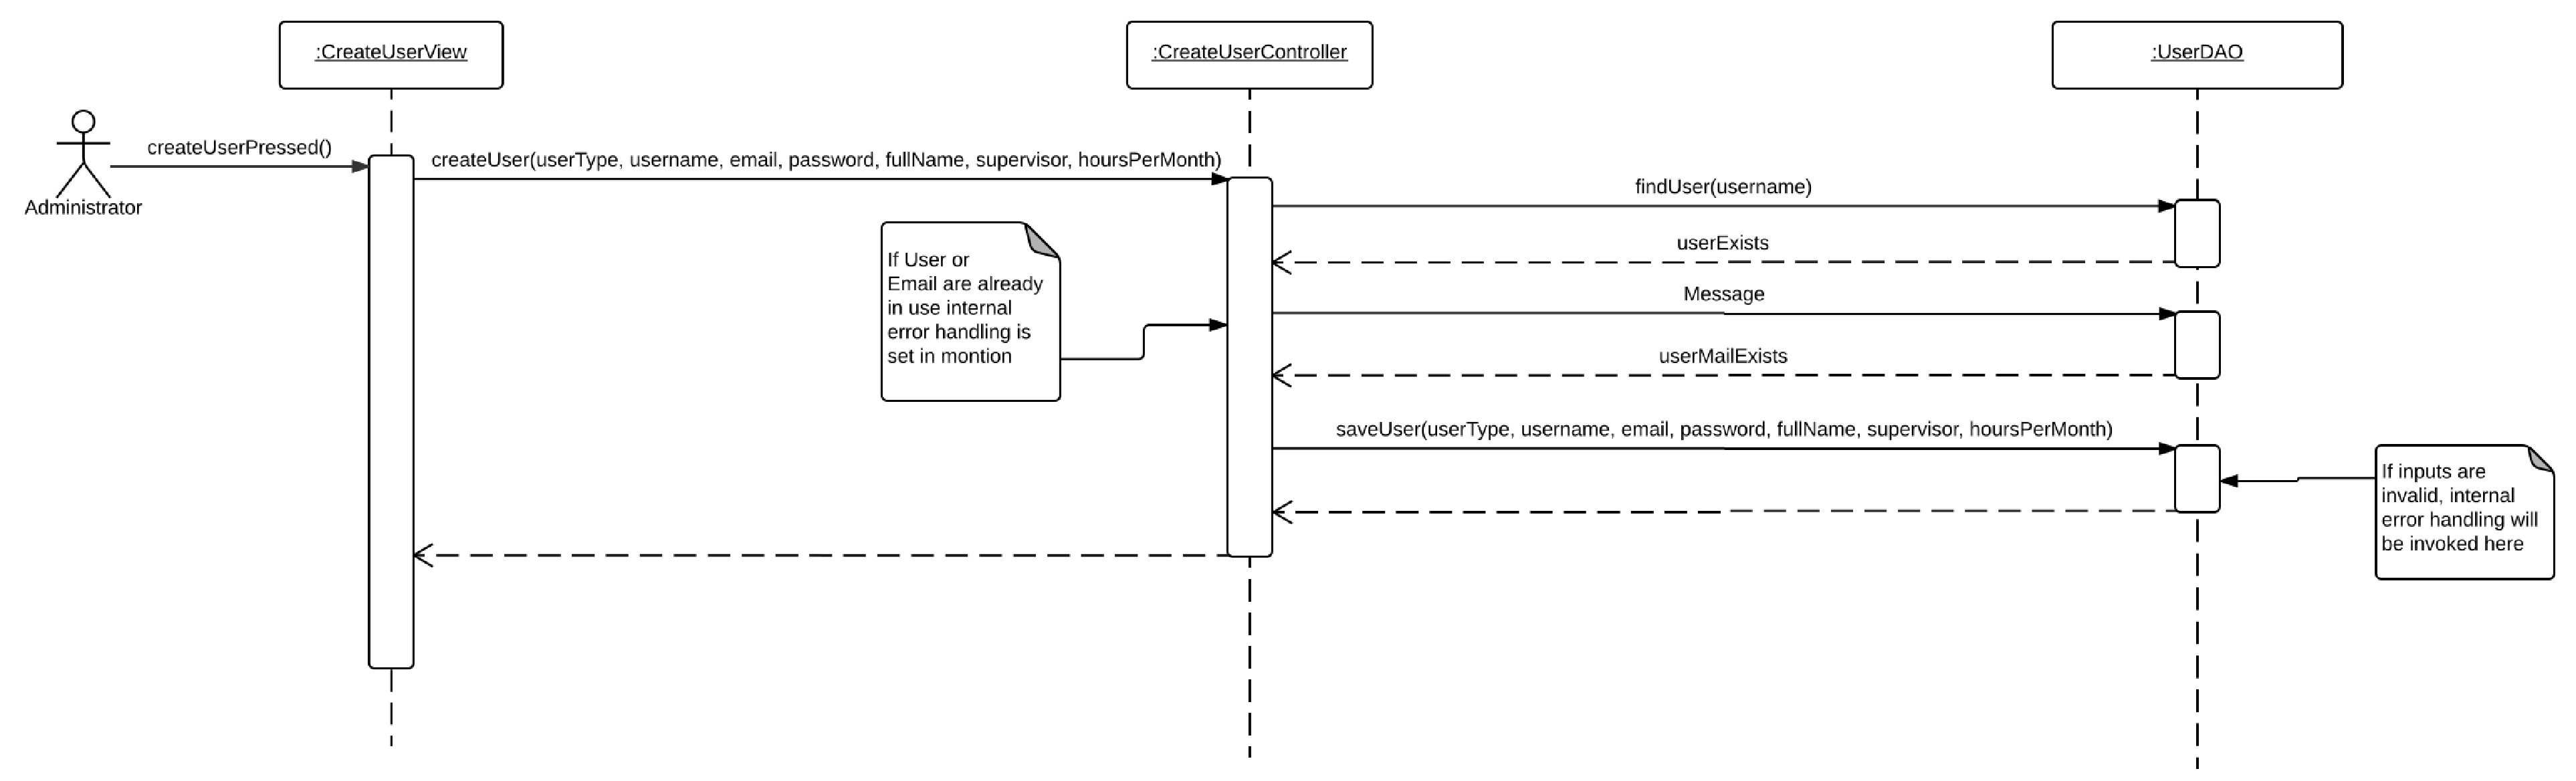
\includegraphics[width=\linewidth]{Create-user-account-new.pdf}
       \caption{Neue Benutzererstellungssequenz}
    \end{figure}

\subsection{Neue Zeiterfassung - Sequenz}

    \begin{figure}
      \centering
        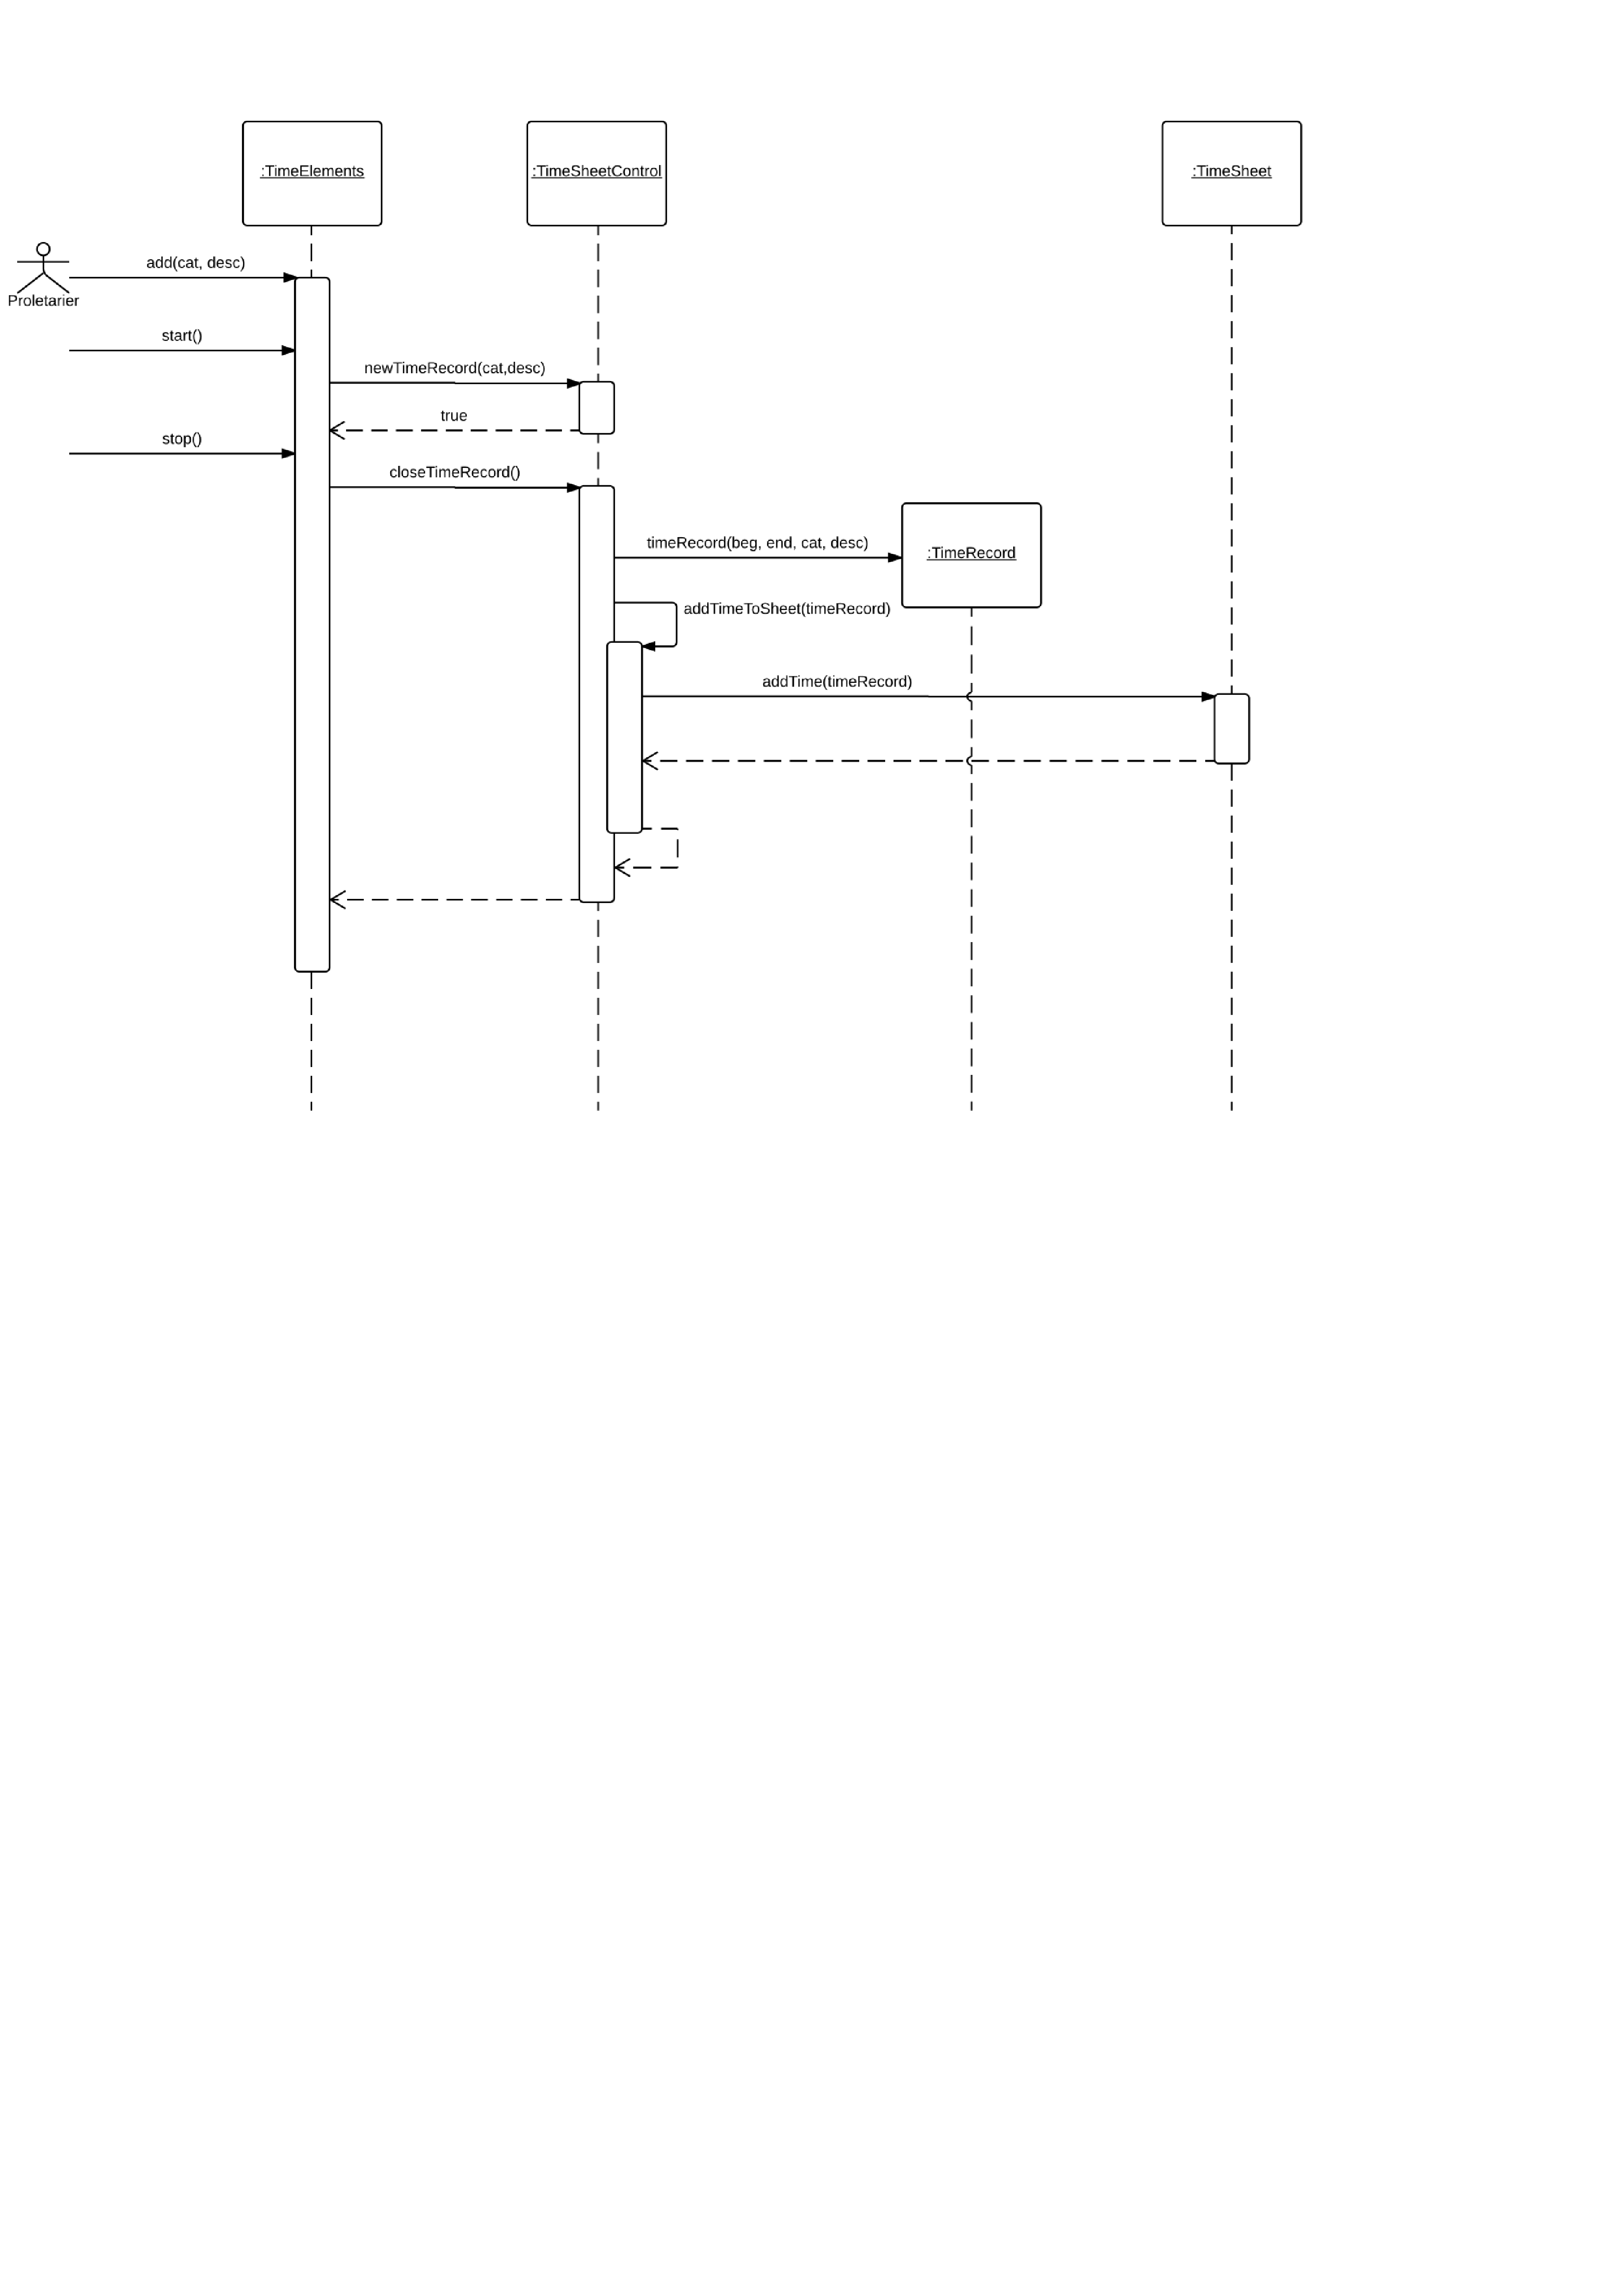
\includegraphics[width=\linewidth]{new-Time-record.pdf}
       \caption{Alte Zeiterfassungssequenz}
    \end{figure}

    \paragraph{Veränderungen}
    \begin{itemize}
        \item Der Ablauf wurde in einklag mit Hibernate gebracht.
        \begin{itemize}
            \item Die TimeSheetControl kommuniziert nurnoch mit dem TimeSheetDAO
            \item TimeRecords werden erstellt und gespeichert, sobald die Zeiterfassung gestartet wurde\(erhöhte persistenz\)
            \item Wird der Tiem record geschlossen wird an dem jüngsten TimeRecord eine Endzeit hinzugefügt.
        \end{itemize}
        \item Das durchreichen von Wahrheitswerten wurde durch internes error handling ersetzt.
    \end{itemize}

    \begin{figure}
      \centering
        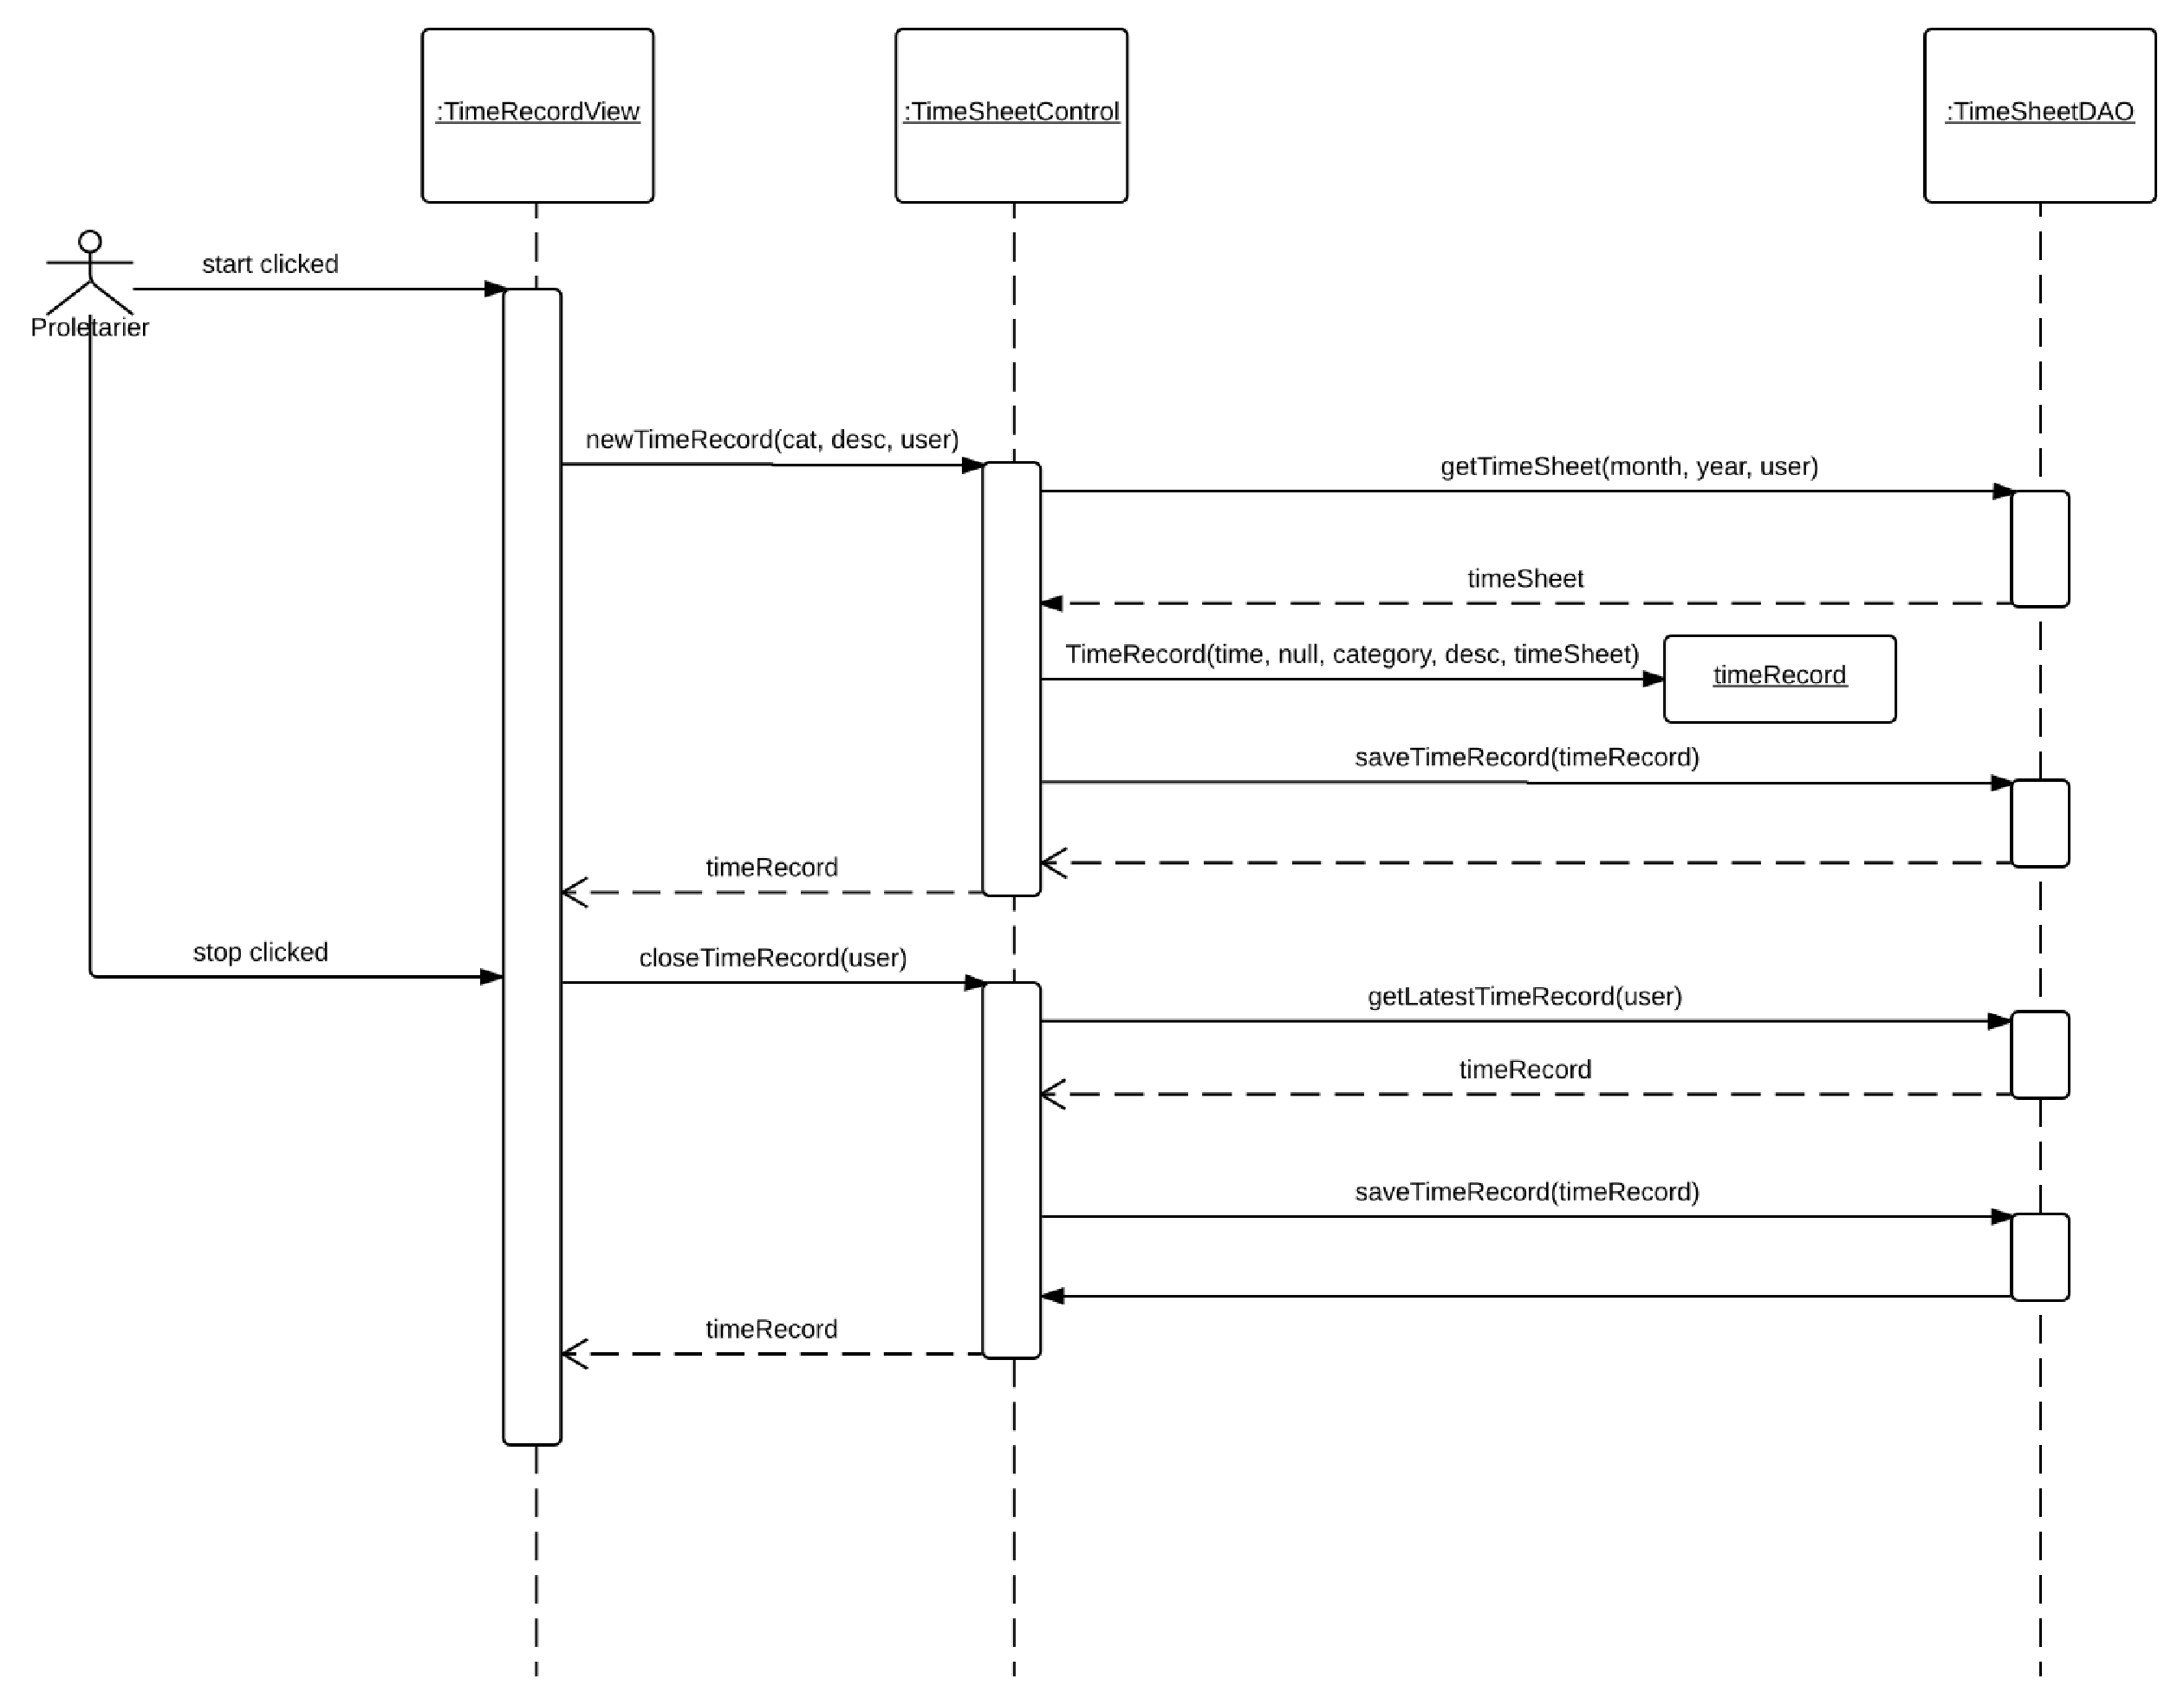
\includegraphics[width=\linewidth]{new-Time-record-new.pdf}
       \caption{Neue Zeiterfassungssequenz}
    \end{figure}

\subsection{Admin druckt alle Stundenzettel - Sequenz}
    \begin{figure}
      \centering
        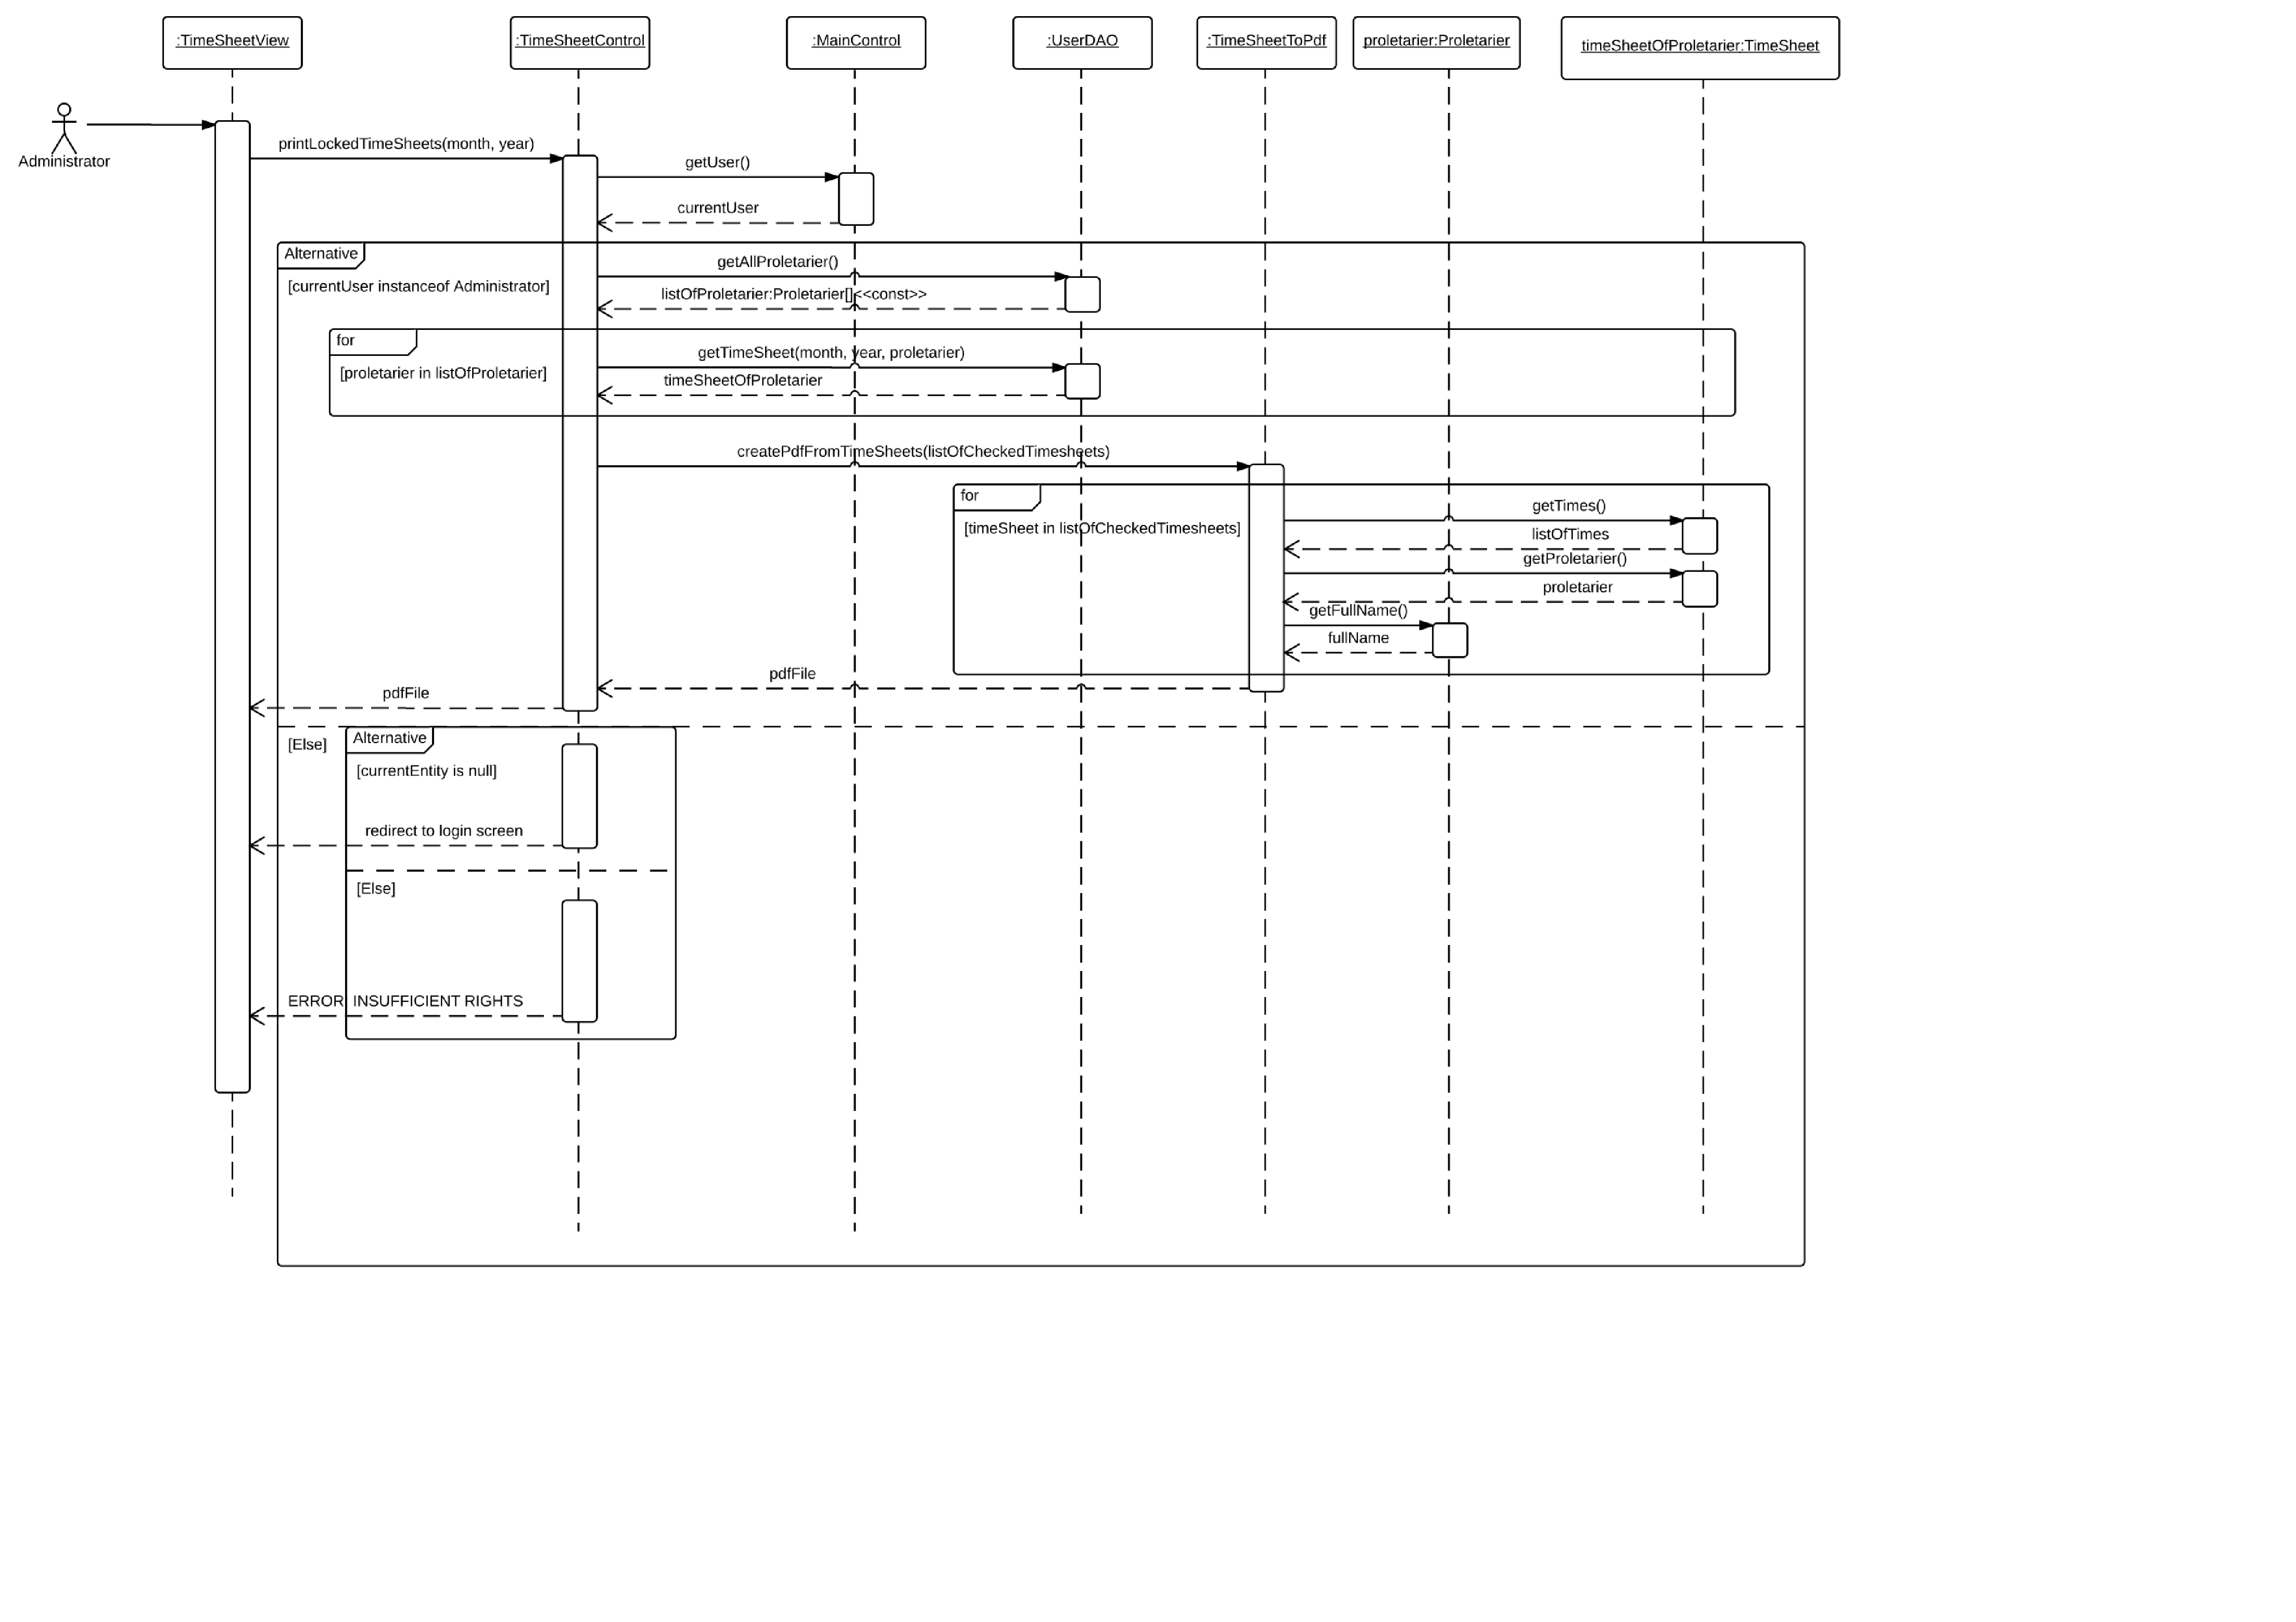
\includegraphics[width=\linewidth]{Admin-prints-all-timesheets.pdf}
       \caption{Alte Admin druckt Sequenz}
    \end{figure}

    \paragraph{Veränderungen}
    \begin{itemize}
        \item Der Ablauf durch Hibernate stark vereinfacht
        \begin{itemize}
            \item Anstatt durch die for Schleifen die Stundezettel iterativ zu sammeln, genügt nun eine SQL abfrage im DAO um alle Stundenzettel zu erhalten
        \end{itemize}
        \item Das drucken übernimmt nun eine Subfunktion des TimeSheetHandlers
    \end{itemize}

    \begin{figure}
      \centering
        %\includegraphics[width=\linewidth]{}
       \caption{Aufgrund der Vereinfachungen durch hibernate ist ein Sequenzdiagramm hier nicht notwendig}
    \end{figure}


    \subsection{Alle Stundenzettel von Nutzer eines Supervisor einholen - Sequenz}

        Wird in der derzeitigen Implementierung nicht benötigt, ist deshalb auch nicht implementiert
        \begin{figure}
          \centering
            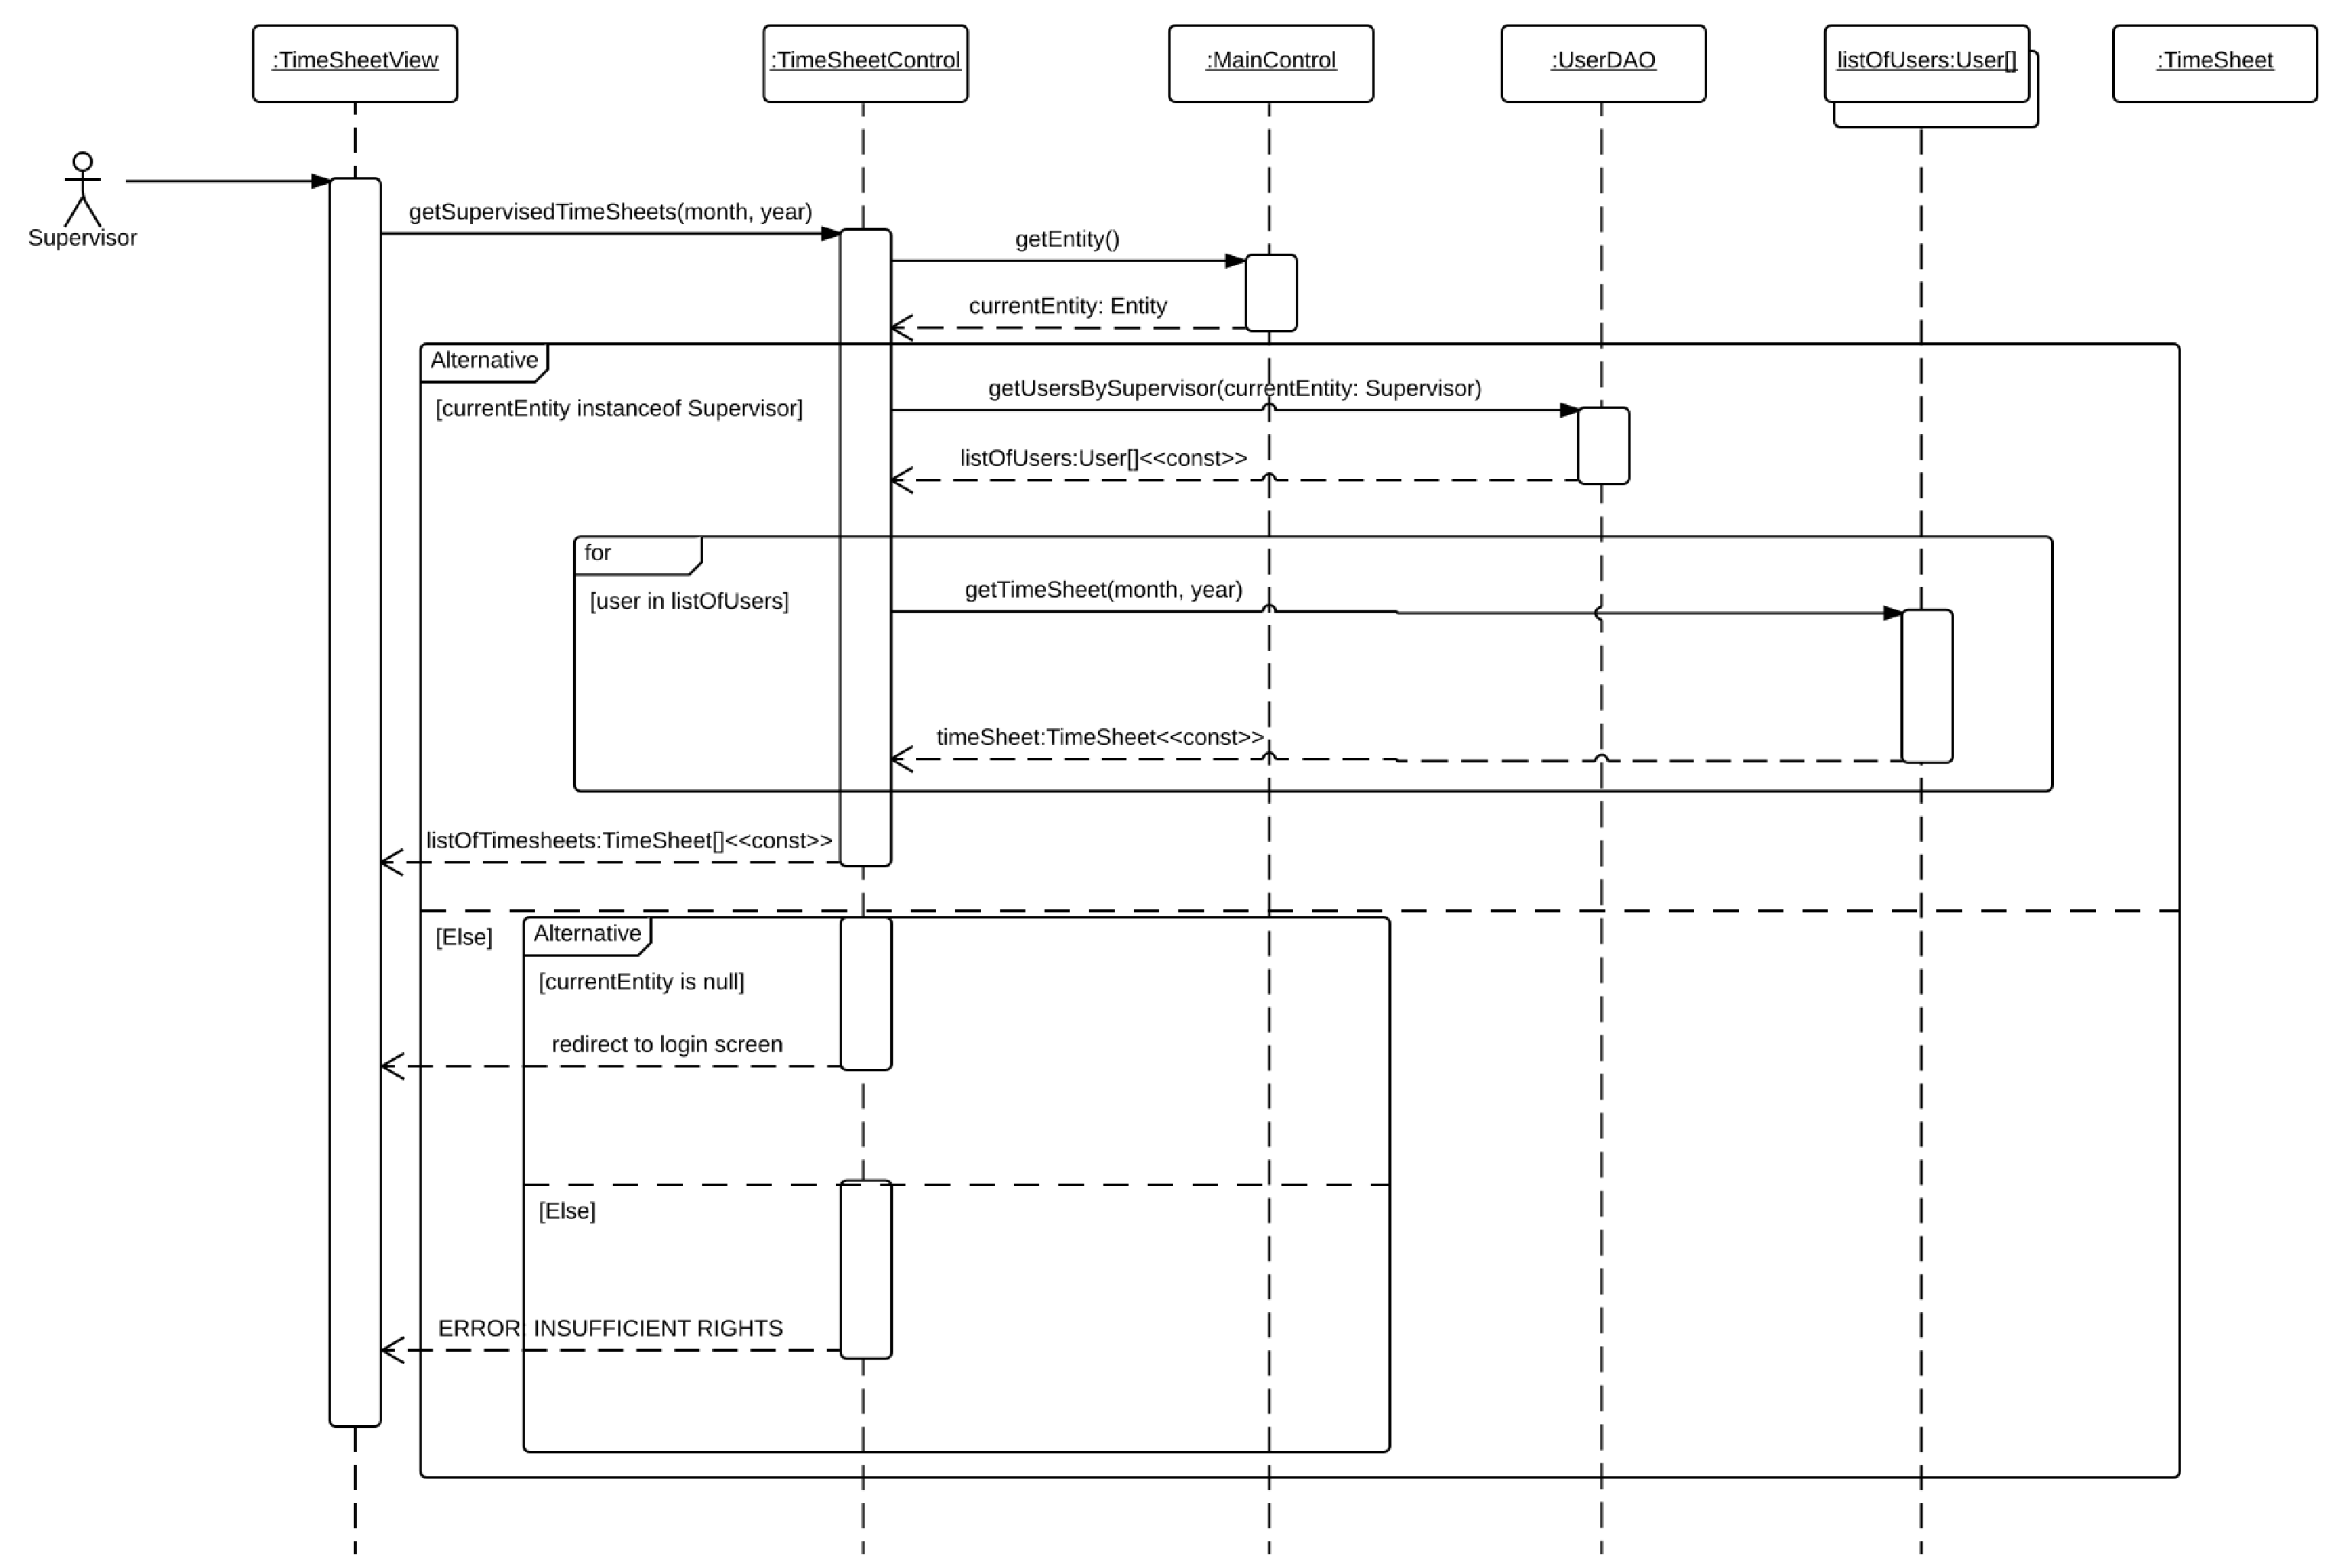
\includegraphics[width=\linewidth]{Get-timesheets-of-all-supervised-users.pdf}
           \caption{Alte Admin druckt Sequenz}
        \end{figure}

        \paragraph{Veränderungen}
        \begin{itemize}
            \item Der Ablauf wäre durch Hibernate stark vereinfacht
            \begin{itemize}
                \item Anstatt durch die for Schleifen die Stundezettel iterativ zu sammeln, genügt nun eine SQL abfrage im DAO um alle Stundenzettel zu erhalten
            \end{itemize}
        \end{itemize}

        \begin{figure}
          \centering
            %\includegraphics[width=\linewidth]{}
           \caption{Aufgrund der Vereinfachungen durch hibernate ist ein Sequenzdiagramm hier nicht notwendig}
        \end{figure}

        \subsection{Nachrichten Versenden und Empfangem - Sequenz}

            \begin{figure}
              \centering
                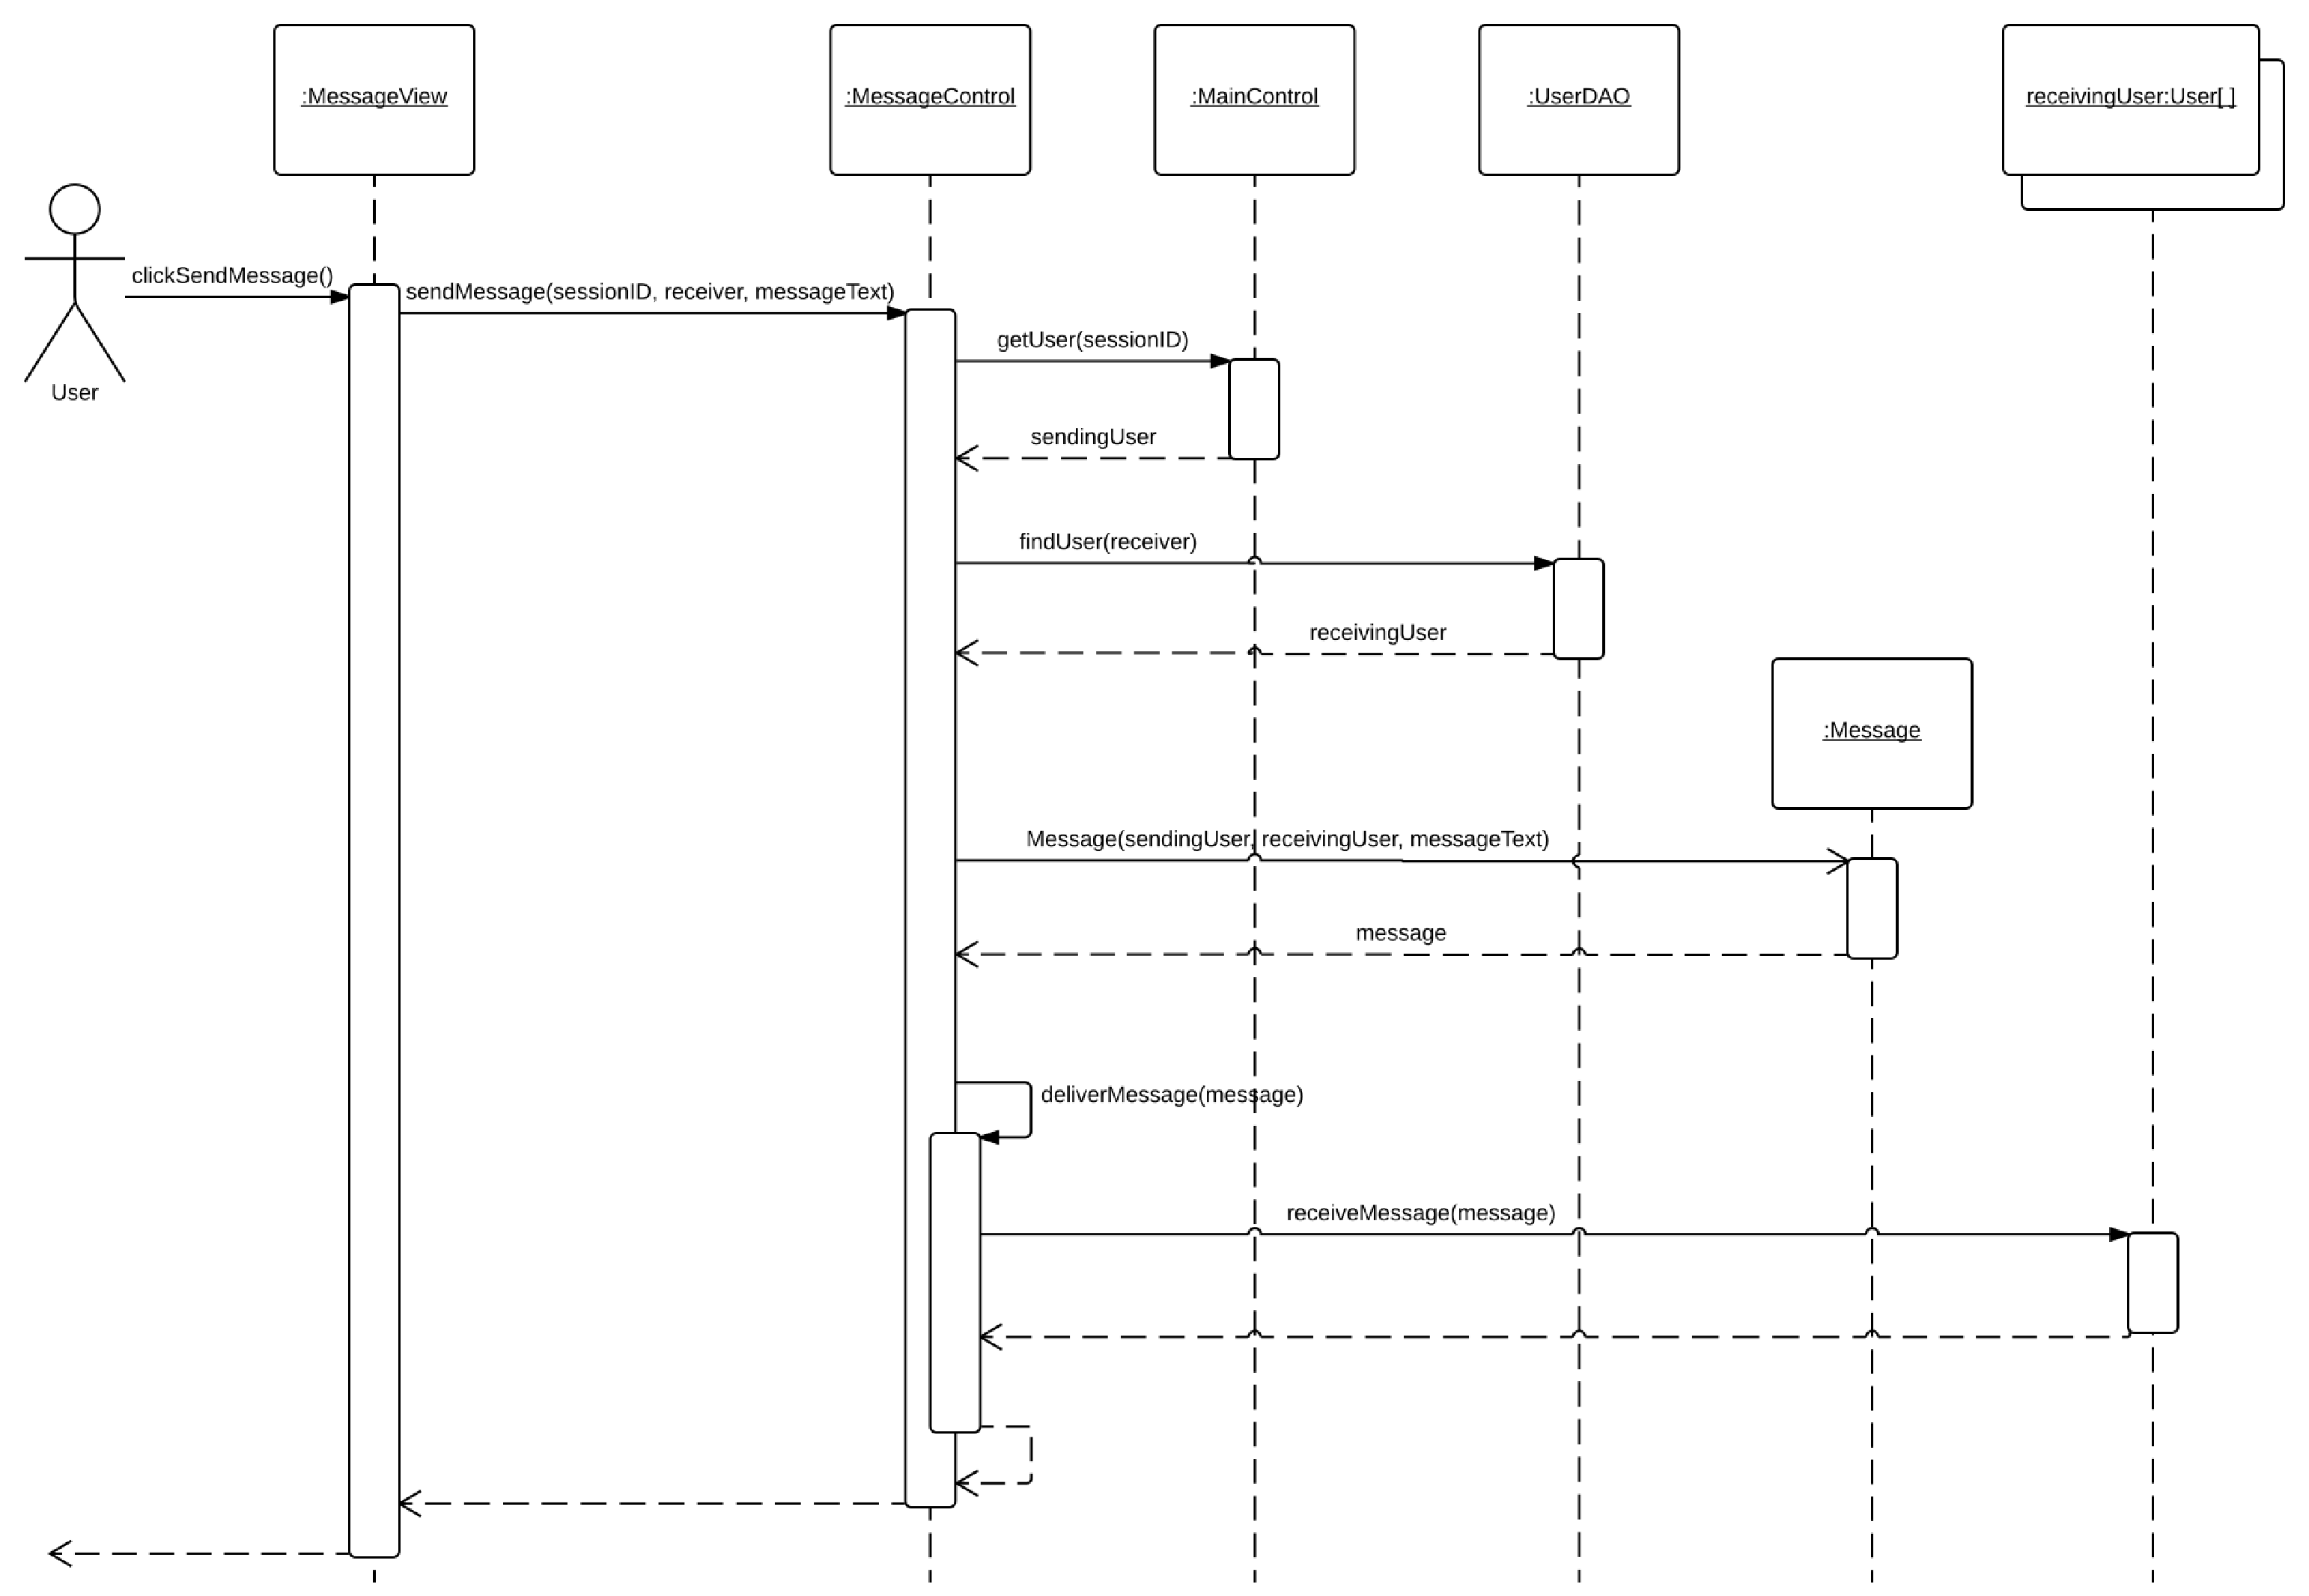
\includegraphics[width=\linewidth]{Message-Delivery.pdf}
               \caption{alte Message Delivery Sequenz}
            \end{figure}

            \paragraph{Veränderungen}
                Durch sich veränderte anforderungen wurde das komplette Message Delivery System obsolet.
            \begin{figure}
              \centering
                %\includegraphics[width=\linewidth]{}
               \caption{Da nichtmehr vorhanden keine neue Version verfügbar}
            \end{figure}


        \subsection{Holen des derzeitigen Timesheets - Sequenz}
            \begin{figure}
              \centering
                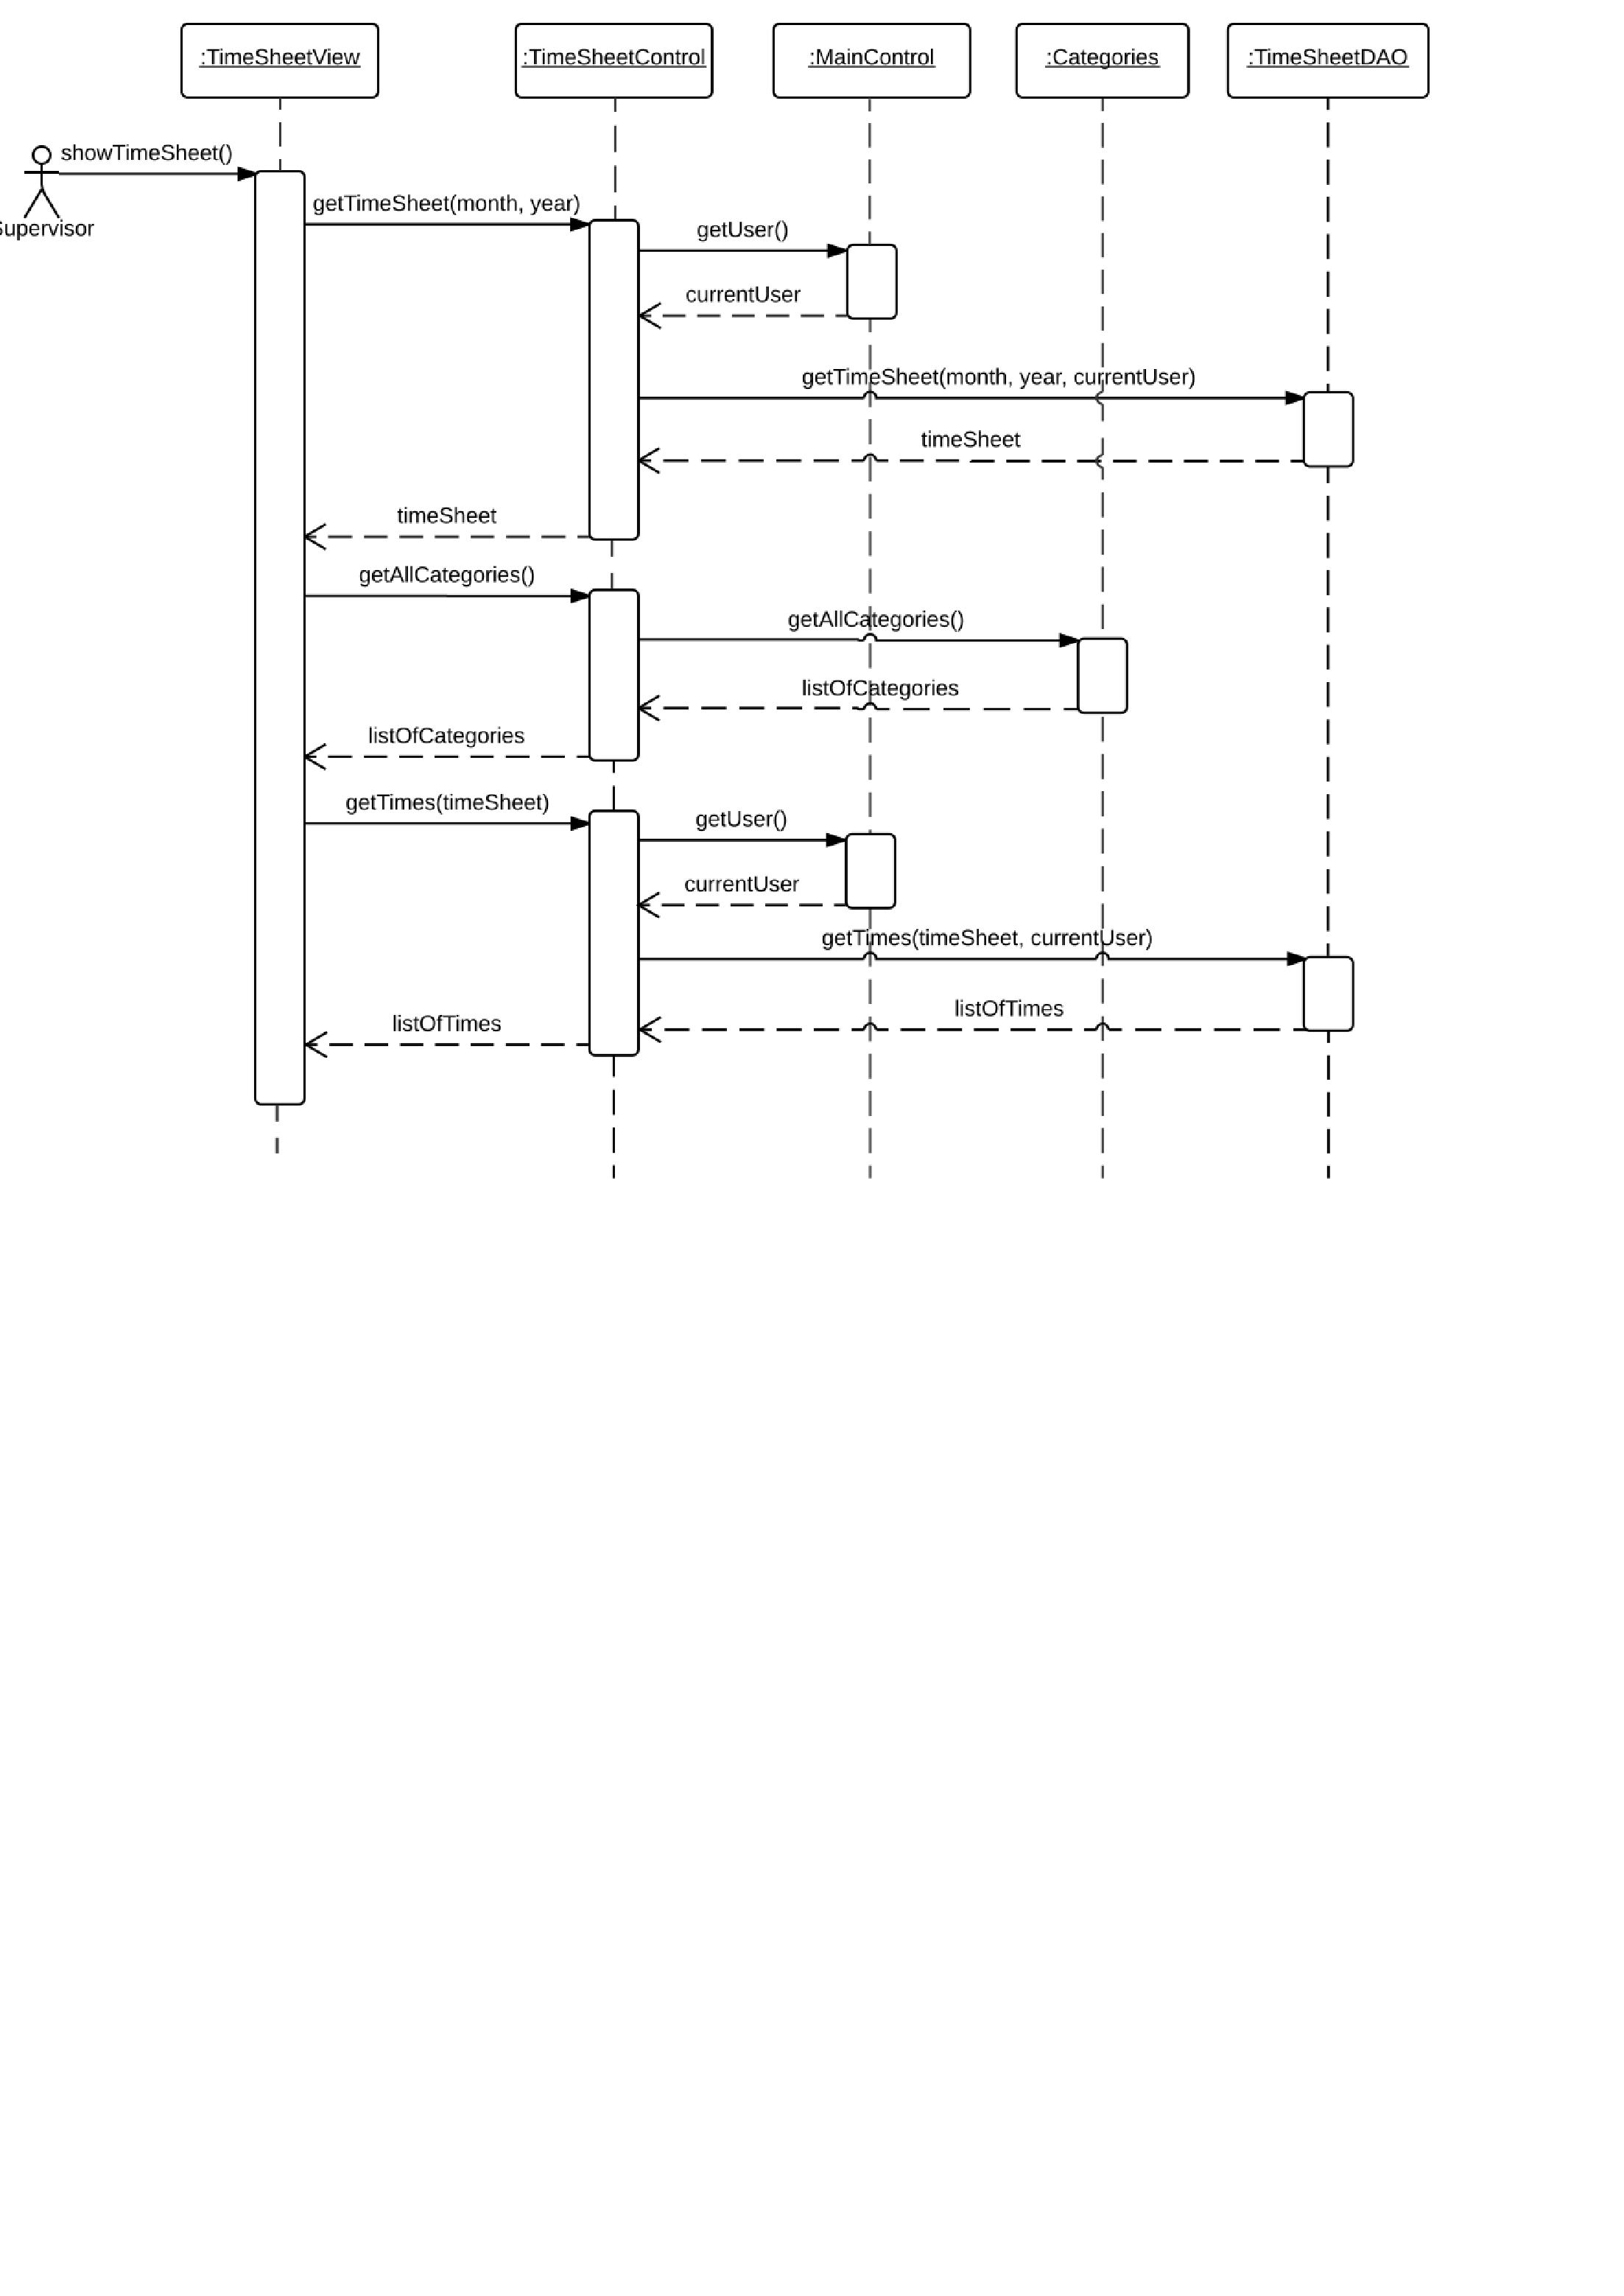
\includegraphics[width=\linewidth]{Get-current-timesheet.pdf}
               \caption{altes Holen des aktuellen timeSheets Sequenz}
            \end{figure}

            \paragraph{Veränderungen}
                Es wird nurnoch ein timeSheet Objekt zur View durchgereicht.
                Diese arbeitet dann intern mit den im Objekt vorhandenen Daten
            \begin{figure}
              \centering
                %\includegraphics[width=\linewidth]{}
               \caption{Keine neue Sequenz notwendig, da stark vereinfacht}
            \end{figure}

        \subsection{Einsenden eines Studenzettels - Sequenz}
                    \begin{figure}
                      \centering
                        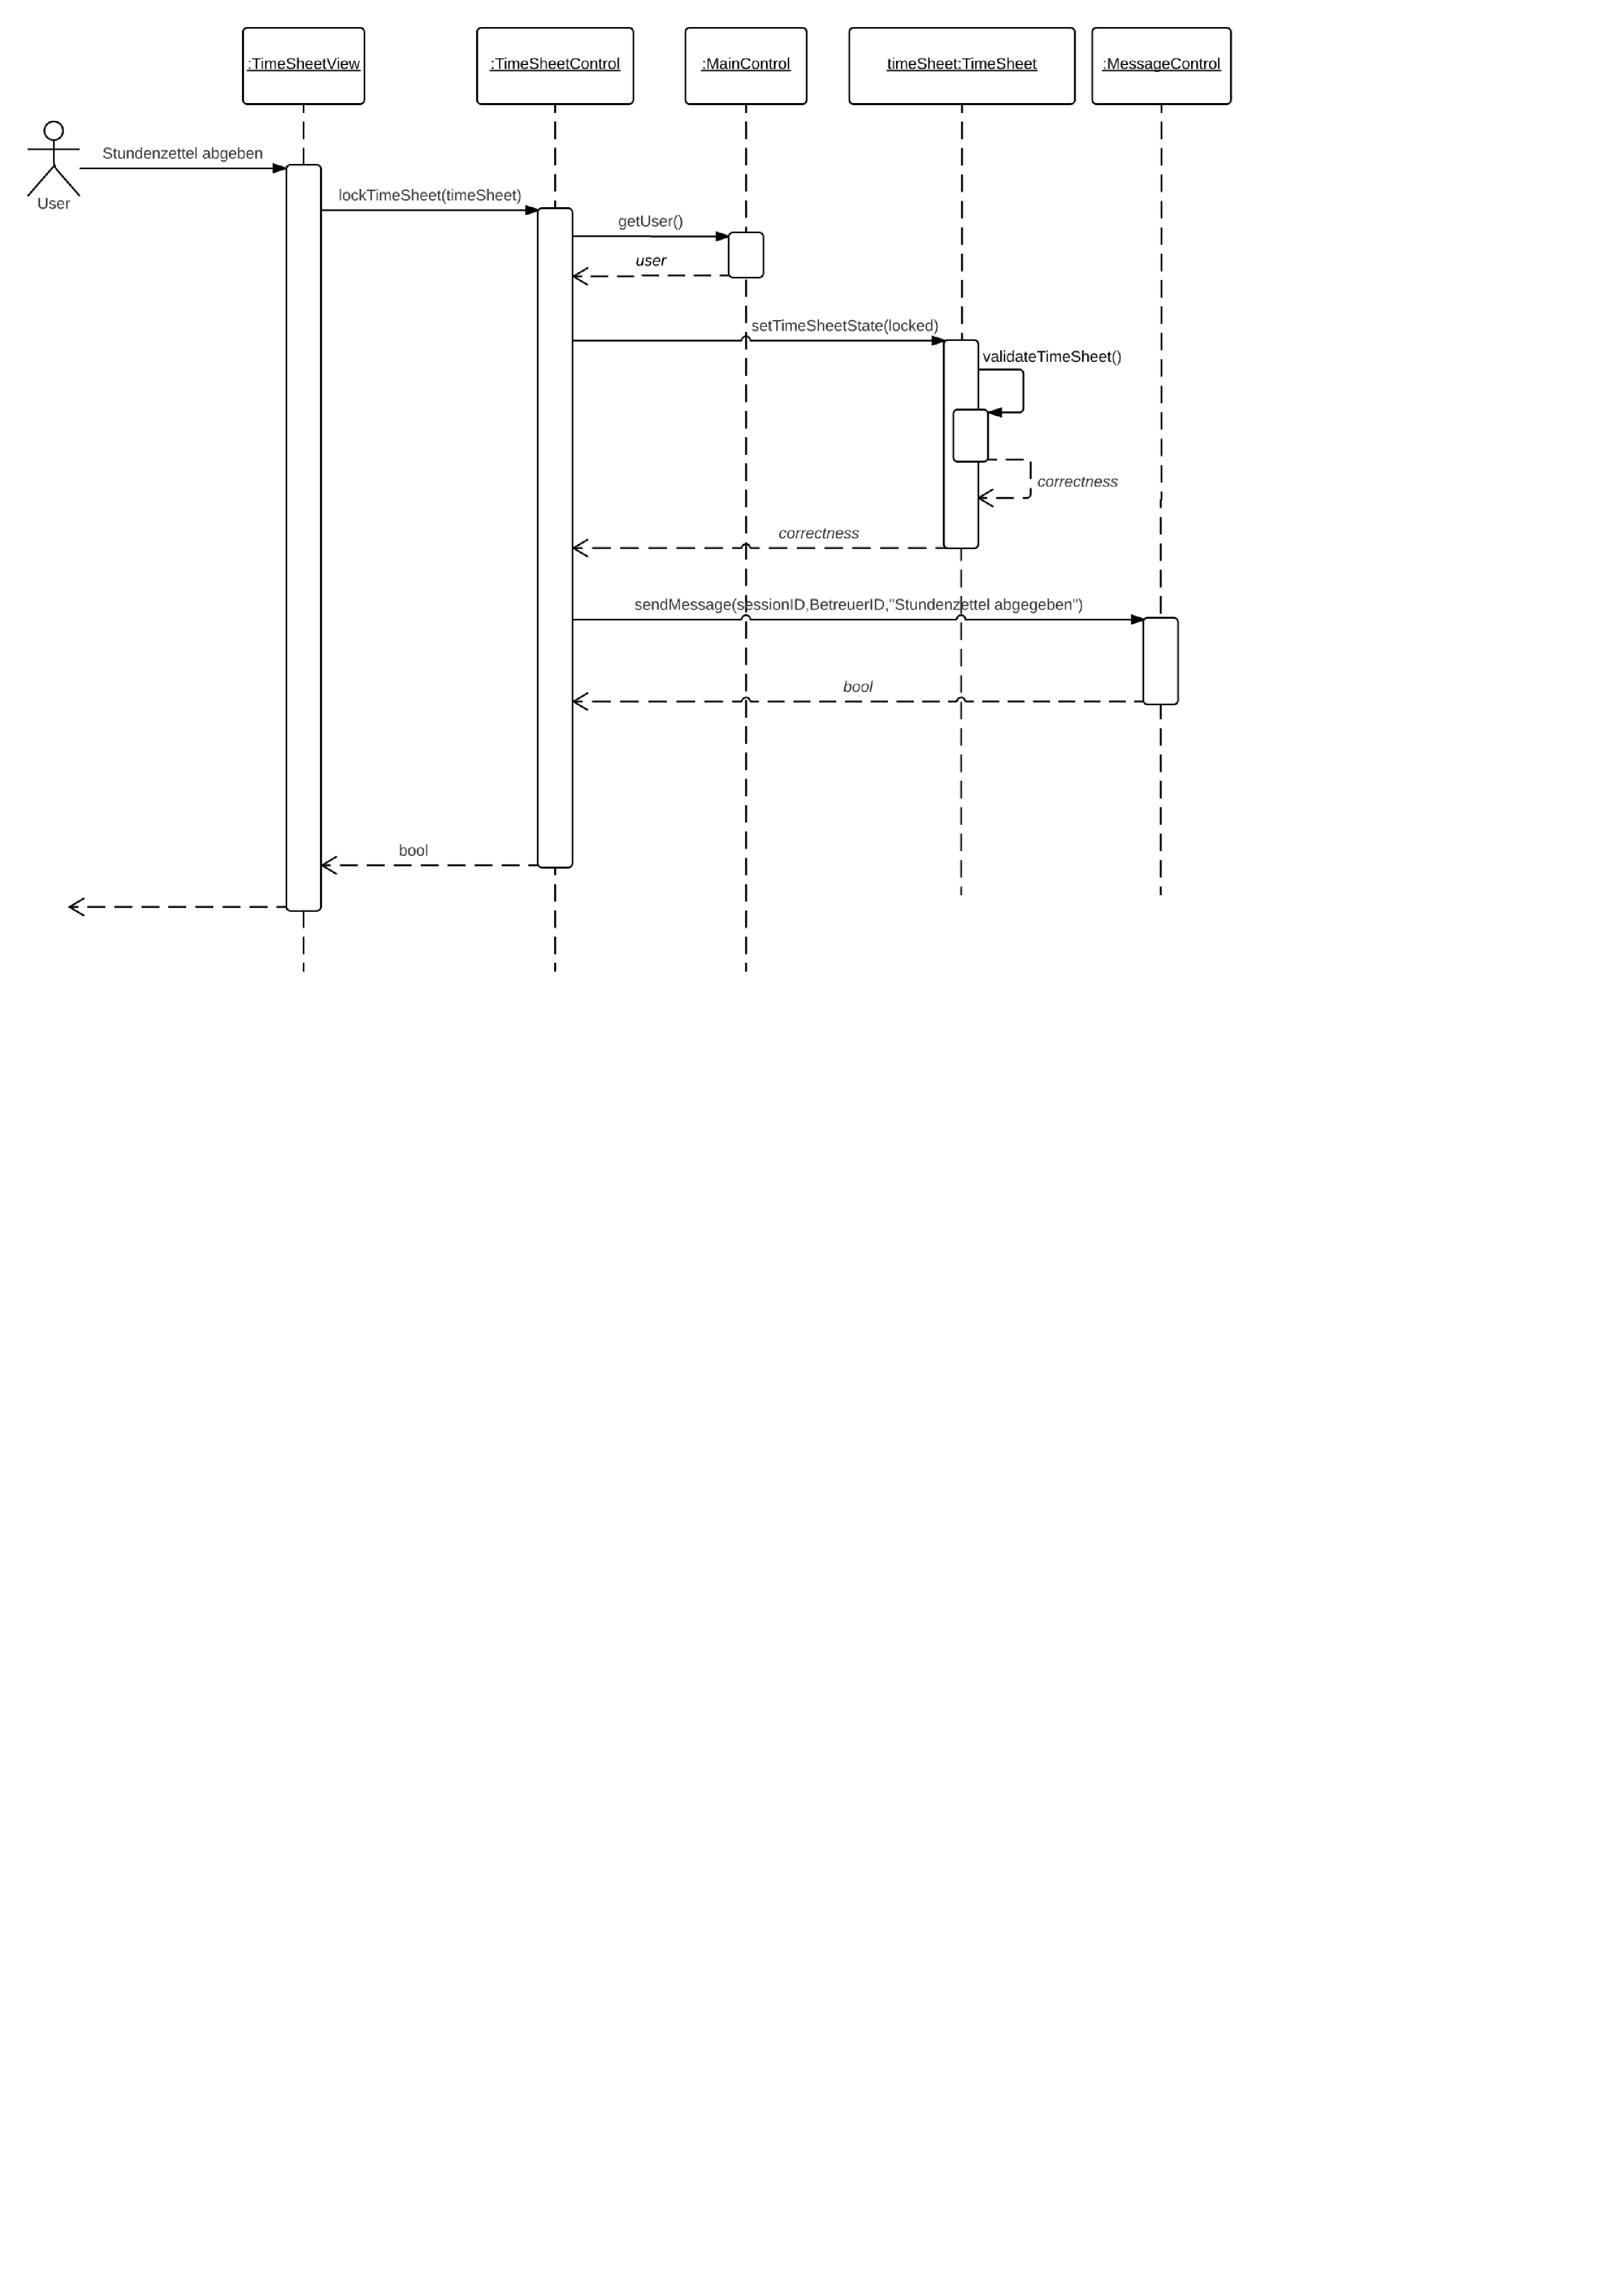
\includegraphics[width=\linewidth]{send-in-timesheet.pdf}
                       \caption{altes einsenden eines fertigen Stundenzettels  Sequenz}
                    \end{figure}

                    \paragraph{Veränderungen}
                    \begin{itemize}
                        \item Keine Benachrichtugungen mehr, da keine interne Nachrichten struktur
                        \item Benachrichtigung wird per EMail versendet
                        \item Das Einsenden wurde mit den \emph{locken} eines TimeSheets vereinfacht
                    \end{itemize}
                    \begin{figure}
                      \centering
                        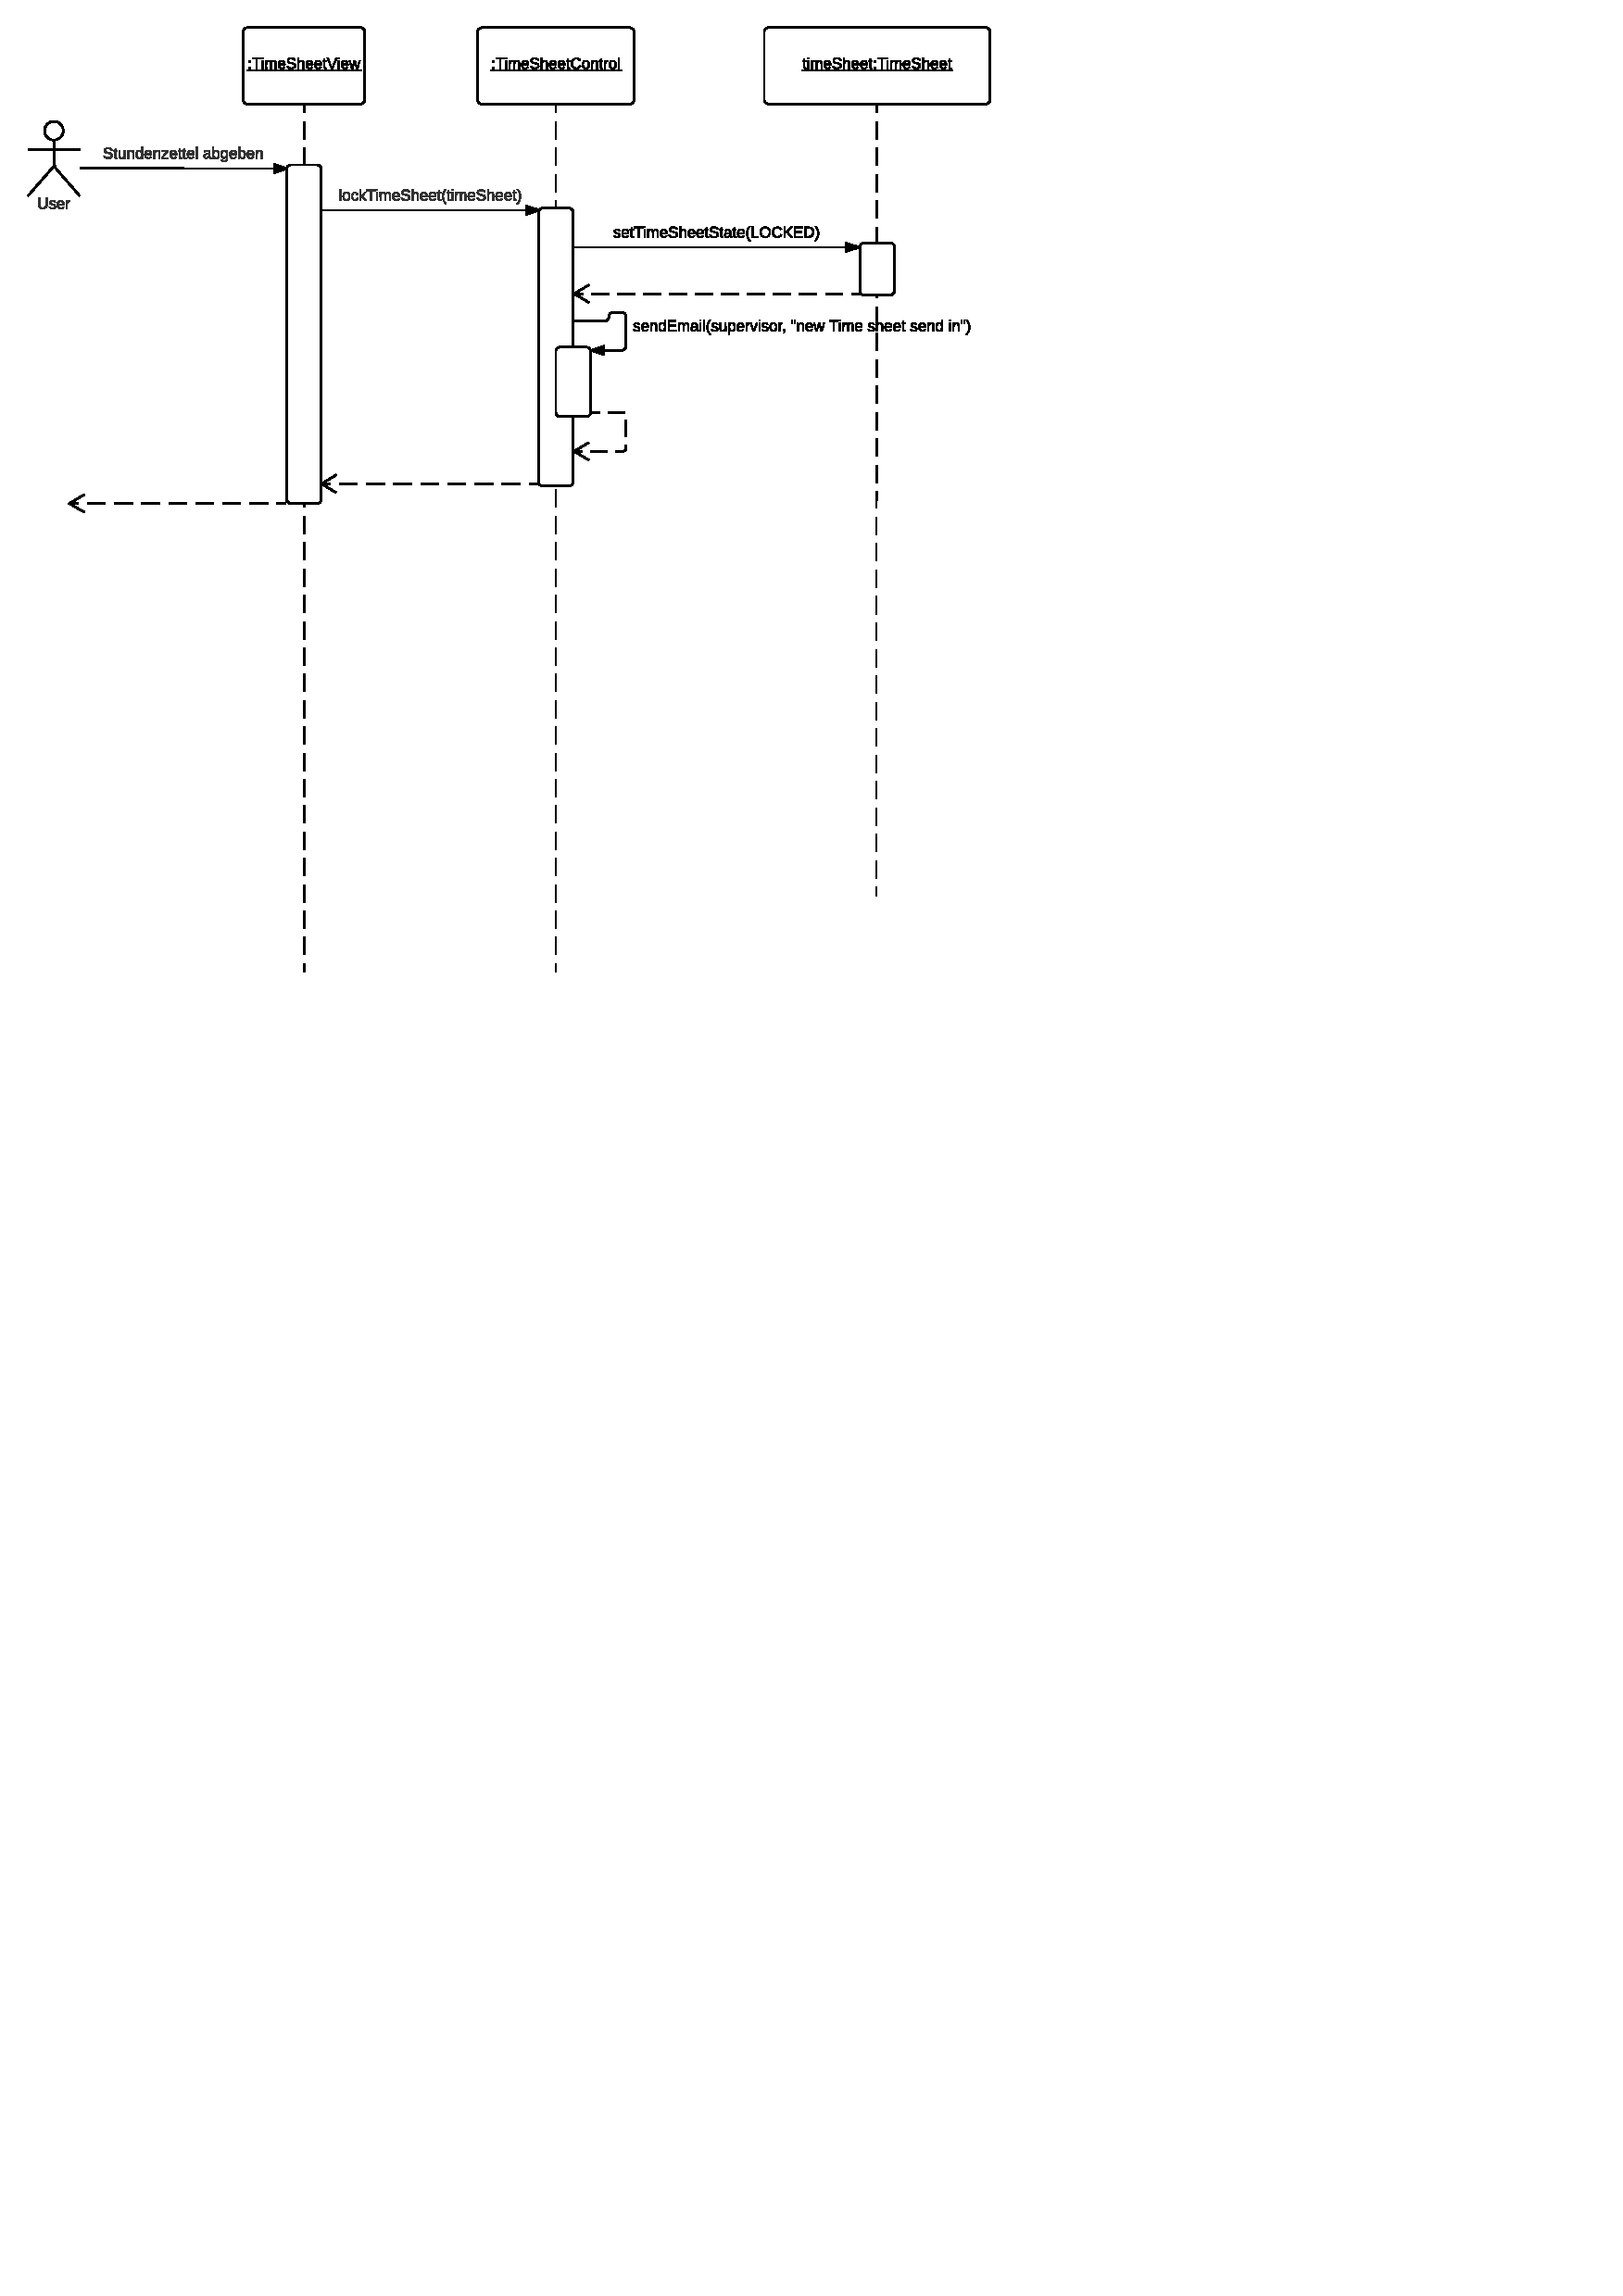
\includegraphics[width=\linewidth]{send-in-timesheet-new.pdf}
                       \caption{neues Einsenden von Stundenzetteln}
                    \end{figure}
